\chapter{Appendix}
\label{app:appendix_A}
The appendix roughly follows the structure of the main thesis. Some of the tables and plots from the intermediate experiments section (Appendix \ref{sec:appendix_A3}) were obtained during an exploratory phase and thus are only approximated and do not contain subject-wise information. However they should give an overview of the logical reasoning that led to the final experiment, for which more individual information is reported in Appendix \ref{sec:appendix_A4}. Individual ROC curves, labels distribution and confusion matrices are only reported for specific examples regarding the unbalance of some datasets (see Appendix \ref{sec:appendix_A3.3})

\section{Pilot study}
\label{sec:appendix_A1}
A pilot study was run internally with myBrainTechnologies employee to design the Experimental Annotator App. The choice of using mouse as input method was evaluated through A\text{\textbar}B testing with two training sessions using a demo of the app. The table reports the average usability score for each training session.

\subsection{Usability scores for ExperimentalAnnotator app demo}
\label{sec:appendix_A1.1}
The usability scores were collected with forms asking to rate how simple it was on a scale from 0 to 5 to perform the following annotation tasks on the GUI representing \ac{VA} space using either the mouse or a joystick:
\begin{itemize}
\item Selecting the desired quadrant 
\item Selecting the perceived emotion
\item Selecting the correct intensity of the perceived emotion
\end{itemize}


\begin{figure}[!htb]
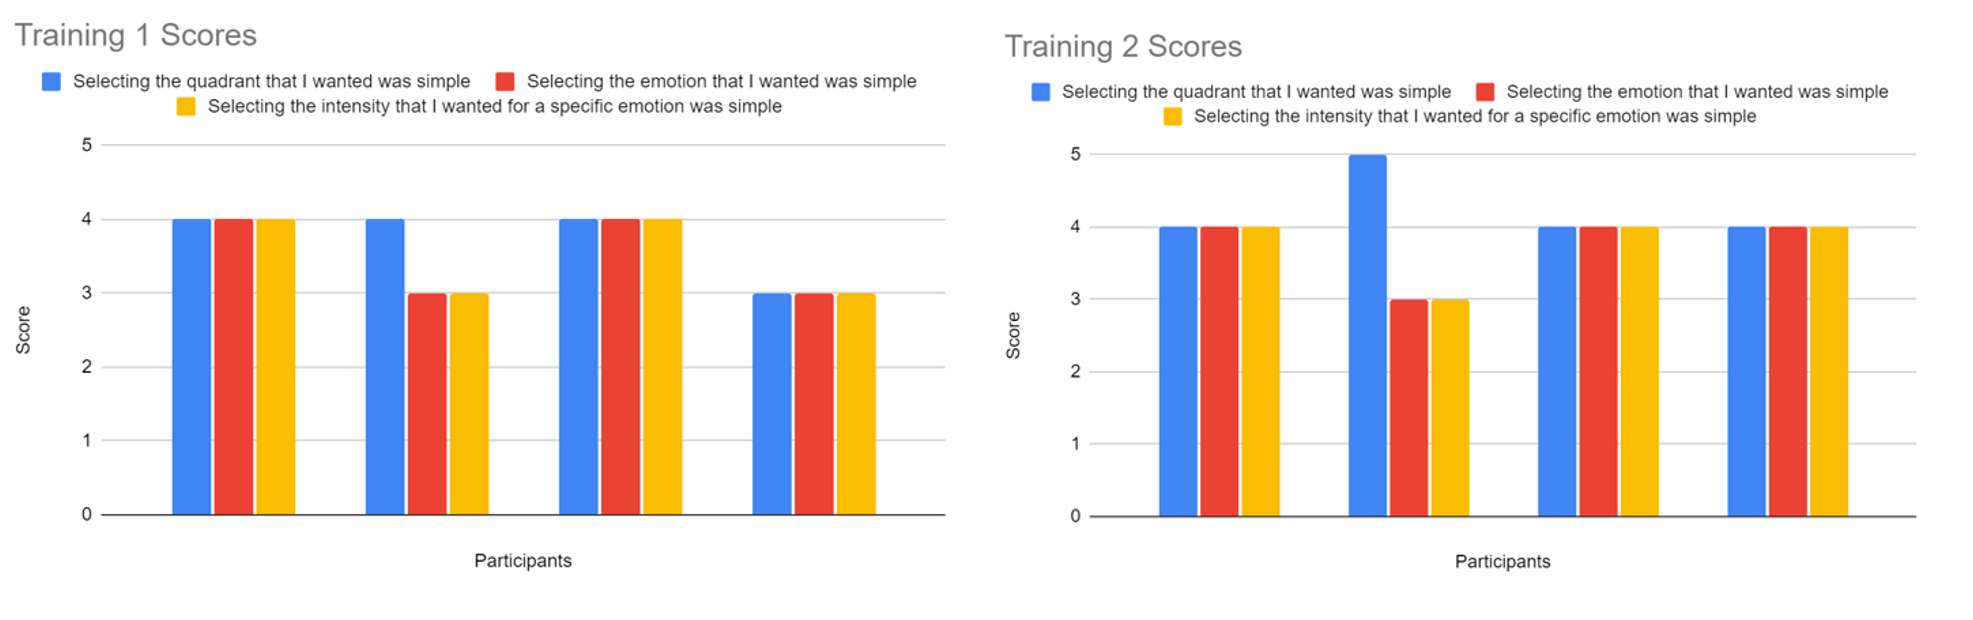
\includegraphics[width=16cm]{img/appendix/usability_condition_A.png}
\centering
\caption{Usability scores for training in condition A (joystick)}\label{fig:usability_condition_A}
\end{figure}

\begin{figure}[!htb]
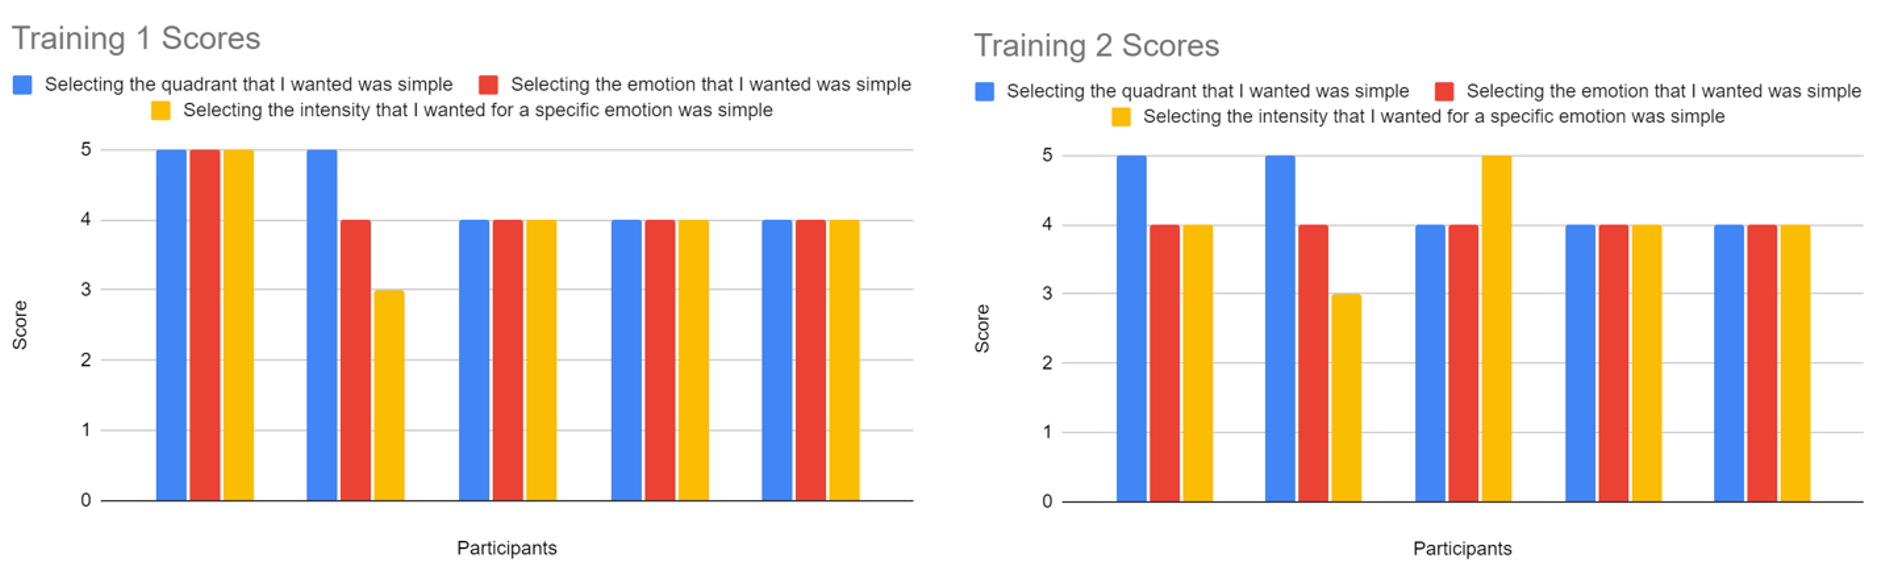
\includegraphics[width=16cm]{img/appendix/usability_condition_B.png}
\centering
\caption{Usability scores for training in condition A (joystick)}\label{fig:usability_condition_B}
\end{figure}
The scores were collected using the training sessions developed for the experiment, so the first training gave the participants some background on the experiment and the task while the second training asked the participants to annotate their emotions in real-time while listening to 4 music excerpts of 30 seconds each. As it can be seen from table \ref{tbl:table_usability__scores}, on average joystick users improved their ability to select what they wanted while mouse users were consistent. This was not completely unexpected since the mouse is very likely to be used by most people working with computers, while joystick is more of a niche input for people who play games or use simulators.

\begin{table}[!htb]
  \caption{Average usability scores for the two groups.}
  \label{tbl:table_usability__scores}
  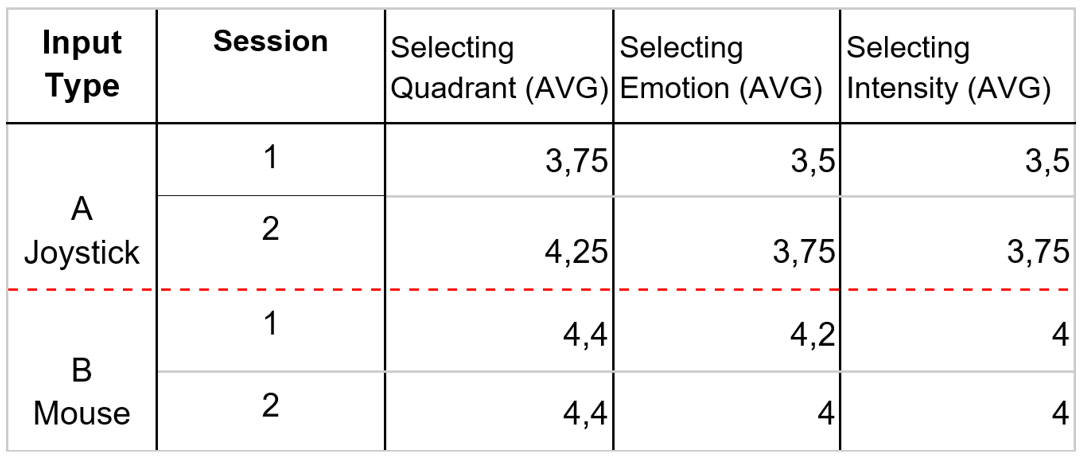
\includegraphics[width=\linewidth]{img/appendix/table_usability_scores.png}
\end{table}
The lower average ratings obtained by the joystick and the higher likelihood of skill gaps between participants was enough to drop the joystick as input method, which was only really interesting for the possibility of annotating emotions in eyes-closed condition.

\section{Methods}
\label{sec:appendix_A2}

\subsection{Participants infographic}
\label{sec:appendix_A2.1}

\begin{figure}[!htb]
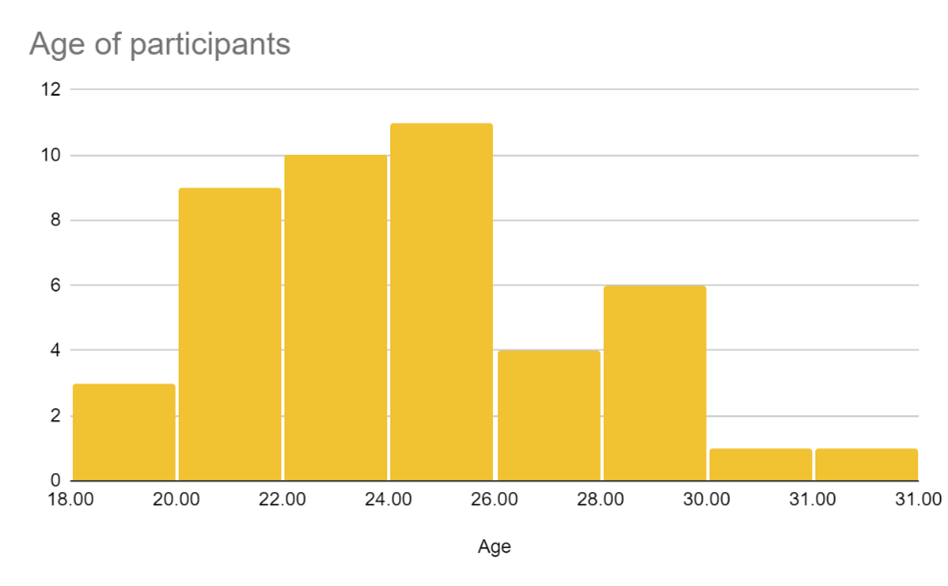
\includegraphics[width=14cm]{img/appendix/age_distribution.png}
\centering
\caption{Age distribution of the population that participated in the experiment}\label{fig:age_distribution}
\end{figure}

\begin{figure}[!htb]
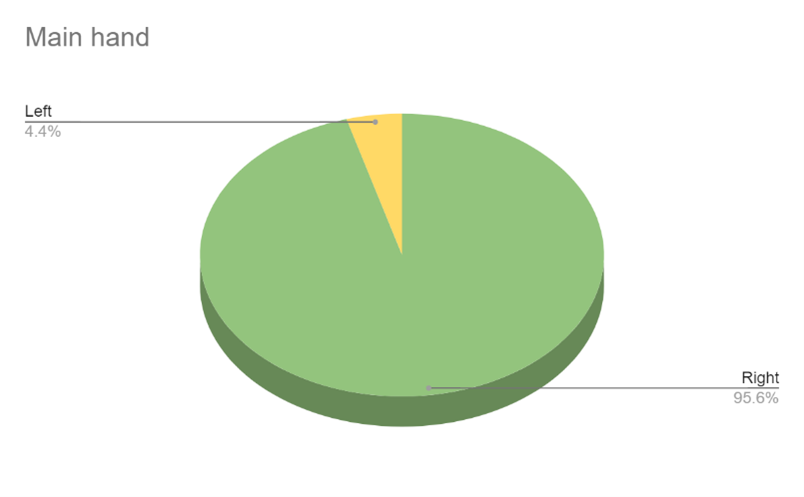
\includegraphics[width=14cm]{img/appendix/right_hand.png}
\centering
\caption{Percentages of right-handed and left-handed over the population that participated in the experiment}\label{fig:right_hand}
\end{figure}

\subsection{Emotion-Music playlist}
\label{sec:appendix_A2.2}
The playlist is a subset of the stimuli proposed by Koelstra et al. \cite{koelstra_deap_2012} and selected using the emotional tagging available on last.fm. The arousal/valence intensity (Low, Medium, High) are a transposition of the scores assigned by users who participated in the web assessment of the aforementioned study, but ultimately have been simplified as a binary representation, low or high.
\\
High Arousal / High Valence (HAHV)
\begin{itemize}
\item  (High arousal, medium positive valence) Excitement- Weapon of choice by Fatboy Slim
\item  (Medium positive arousal, high valence) Happiness - Love Today by Mika
\end{itemize}

Low Arousal / High Valence (LAHV)
\begin{itemize}
\item  (Medium negative Arousal, high valence) Satisfaction - Nasty Naughty Boy, by Christina Aguilera
\item 	 (Low arousal, medium positive valence) Relaxation – Amber by 311
\end{itemize}

Low Arousal / Low Valence (LALV)
\begin{itemize}
\item  (Medium negative arousal, High negative valence) Depression - Last Flowers by Radiohead
\item  (Low arousal, Medium negative valence) Sadness – Hurt by Johnny Cash
\end{itemize}

High Arousal / Low Valence (HALV)
\begin{itemize}
\item  (Medium positive arousal, High negative valence) Anger – Threshold by Slayer
\item  (High positive arousal, Medium negative valence) Anxiety - Trapped Under Ice by Believe
\end{itemize}

Other songs were used in the training sessions, but no labelling is provided as their only purpose was 
to teach the users how to use the EA app GUI.
\begin{itemize}
\item  The white stripes - Seven Nation Army
\item  Gary Jules - Mad World
\item  Oren Lavie - Her morning elegance
\item  The Cranberries - Zombie
\item  Maneskin - I wanna be your slave
\item  Rage against the machine - Killing in the name of
\end{itemize}



\section{Intermediate experiments}
\label{sec:appendix_A3}
During the development of the classification pipeline, several intermediate experiments were run to
explore the data, the methodologies, and the different classifiers. The dataset of each subject was 
explored singularly, but only some examples are reported below

\subsection{Subject-dependent experiment with Sequential Features Selection}
\label{sec:appendix_A3.1}
Sequential Features Selection is a greedy features selection method used to reduce the amount of features by preferring those that improve the performances of a classifier while reducing the variance. Before computing \ac{SFS}, GridSearch was used on the entire dataset including all participants to select the best subject-independent hyperparameters (tables \ref{tbl:mlp_initial_parameters} and \ref{tbl:svm_initial_parameters}). 
\begin{table}[h!]
  \caption{Manually tuned hyper-paramters for MLP.}
  \label{tbl:mlp_initial_parameters}
  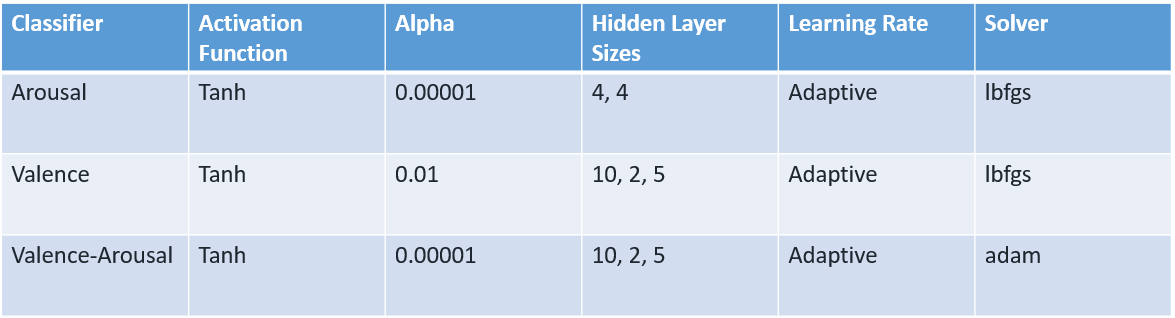
\includegraphics[width=\linewidth]{img/appendix/mlp_initial_parameters.png}
\end{table}

\begin{table}[h!]
  \caption{Manually tuned hyper-paramters for SVM.}
  \label{tbl:svm_initial_parameters}
  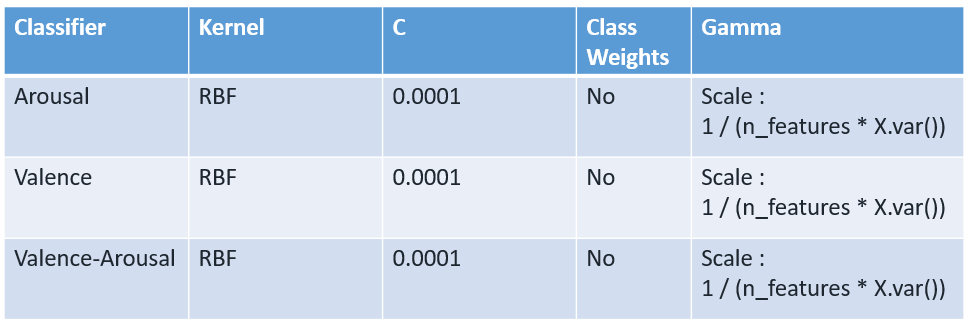
\includegraphics[width=\linewidth]{img/appendix/svm_initial_parameters.png}
\end{table}

\FloatBarrier
Then, forward \ac{SFS} was used to select 5 features for each participant  and perform the first  classification experiment with subject-dependent strategy for each type of classifier (\ac{SVM} or \ac{MLP}) and each condition (EO, EC or EO\&EC). Cross-validated accuracy scores were averaged and reproted in \ref{tbl:sfs_cv_experiment}.

\begin{table}[h!]
  \caption{Average cross-validated accuracy for each classifier and listening condition using SFS.}
  \label{tbl:sfs_cv_experiment}
  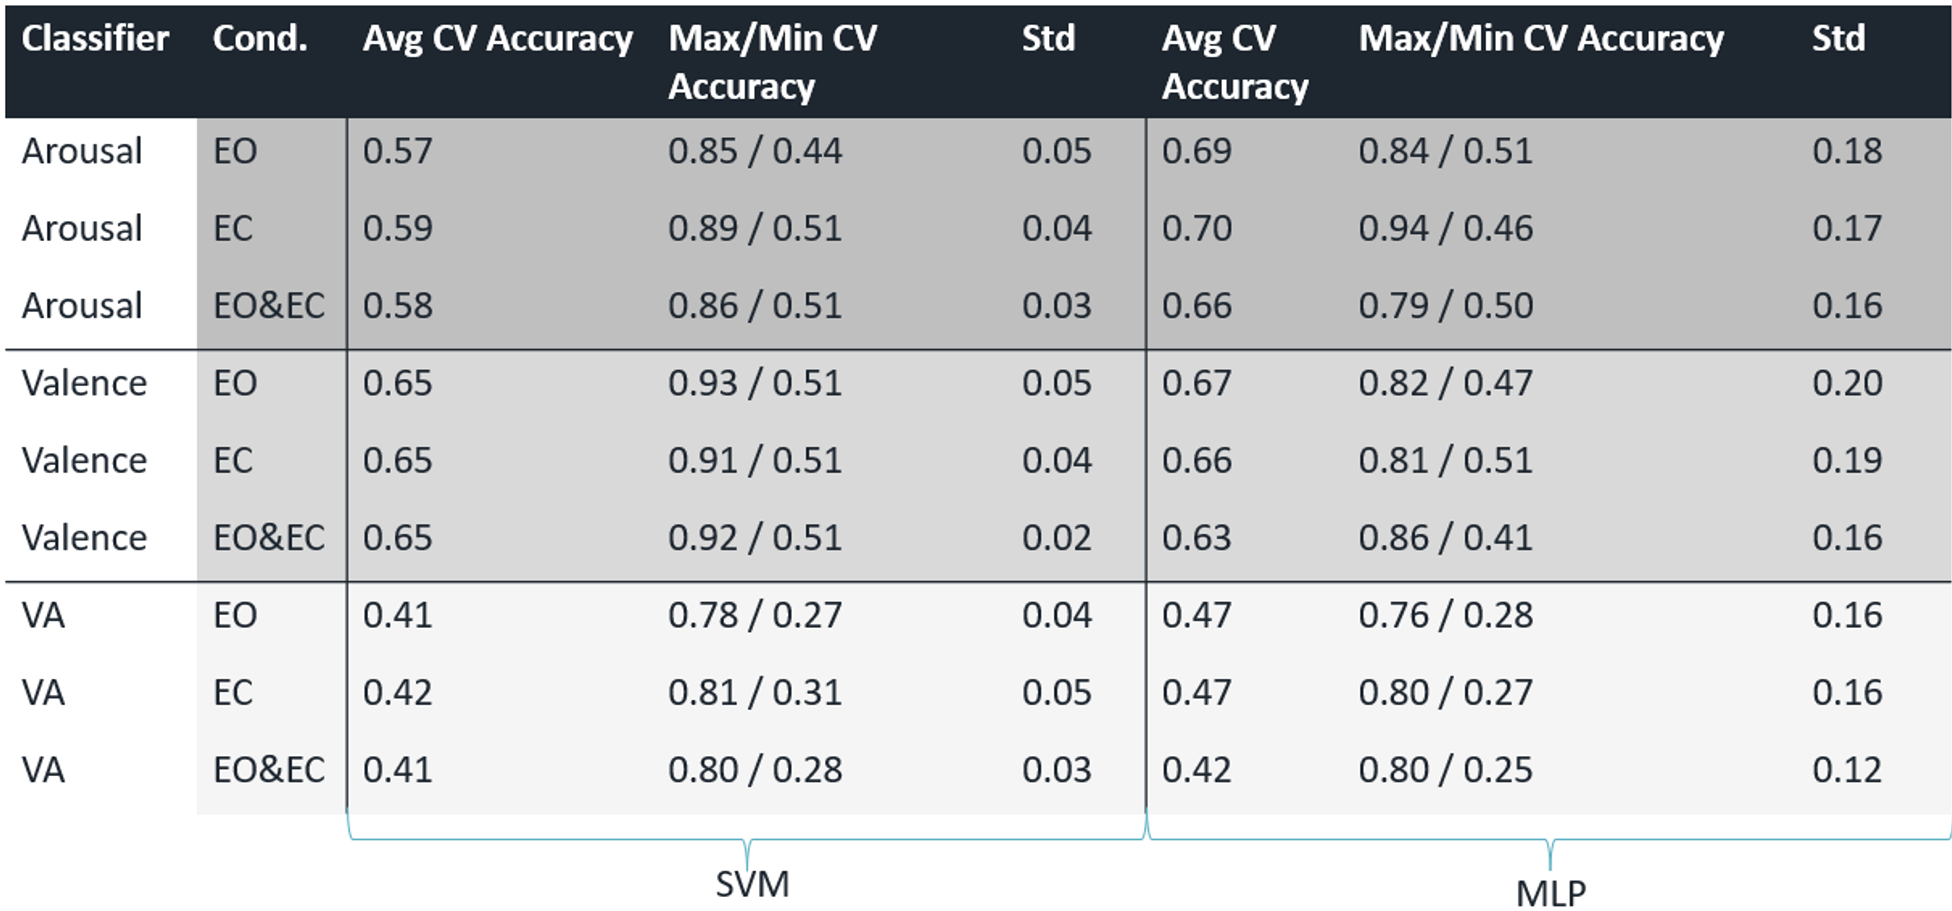
\includegraphics[width=\linewidth]{img/appendix/sfs_cv_experiment.png}
\end{table}

\FloatBarrier
In addition, the most selected features for each classifier and each condition were grouped (see table \ref{tbl:sfs_features}) for later use in two more experiments under the name of TOP5 features.

\begin{table}[h!]
  \caption{Most frequently selected features using SFS, renamed TOP5 features.}
  \label{tbl:sfs_features}
  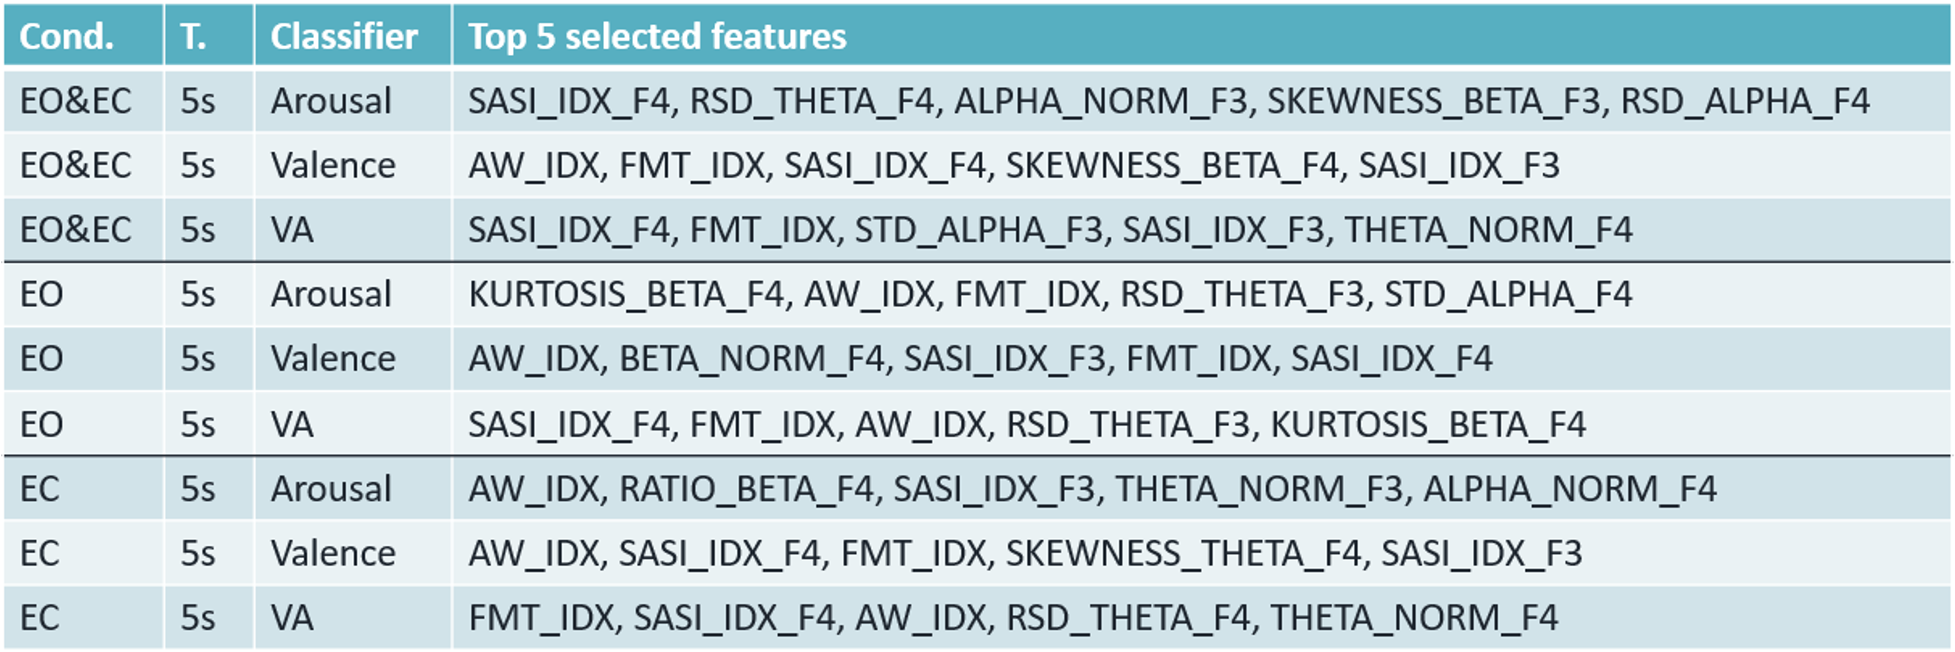
\includegraphics[width=\linewidth]{img/appendix/sfs_features.png}
\end{table}
\FloatBarrier

\subsection{Subject-dependent experiment with TOP5 features}
\label{sec:appendix_A3.2}
For this experiment, the average TOP5 features selected using \ac{SFS} were applied to all the generated models, for each classification task and in each condition similarly to the previous experiment. Average CV accuracy scores were lower, suggesting that applying the same features using this generalization criterion was not optimal for subject-dependent strategy. For this reason, and to optimize computational time, the dimensionality of the features array was later reduced using \ac{PCA} instead in the final experiments.

\begin{table}[h!]
  \caption{Average cross-validated accuracy for each classifier and listening condition using TOP5 features.}
  \label{tbl:top5_cv_experiment}
  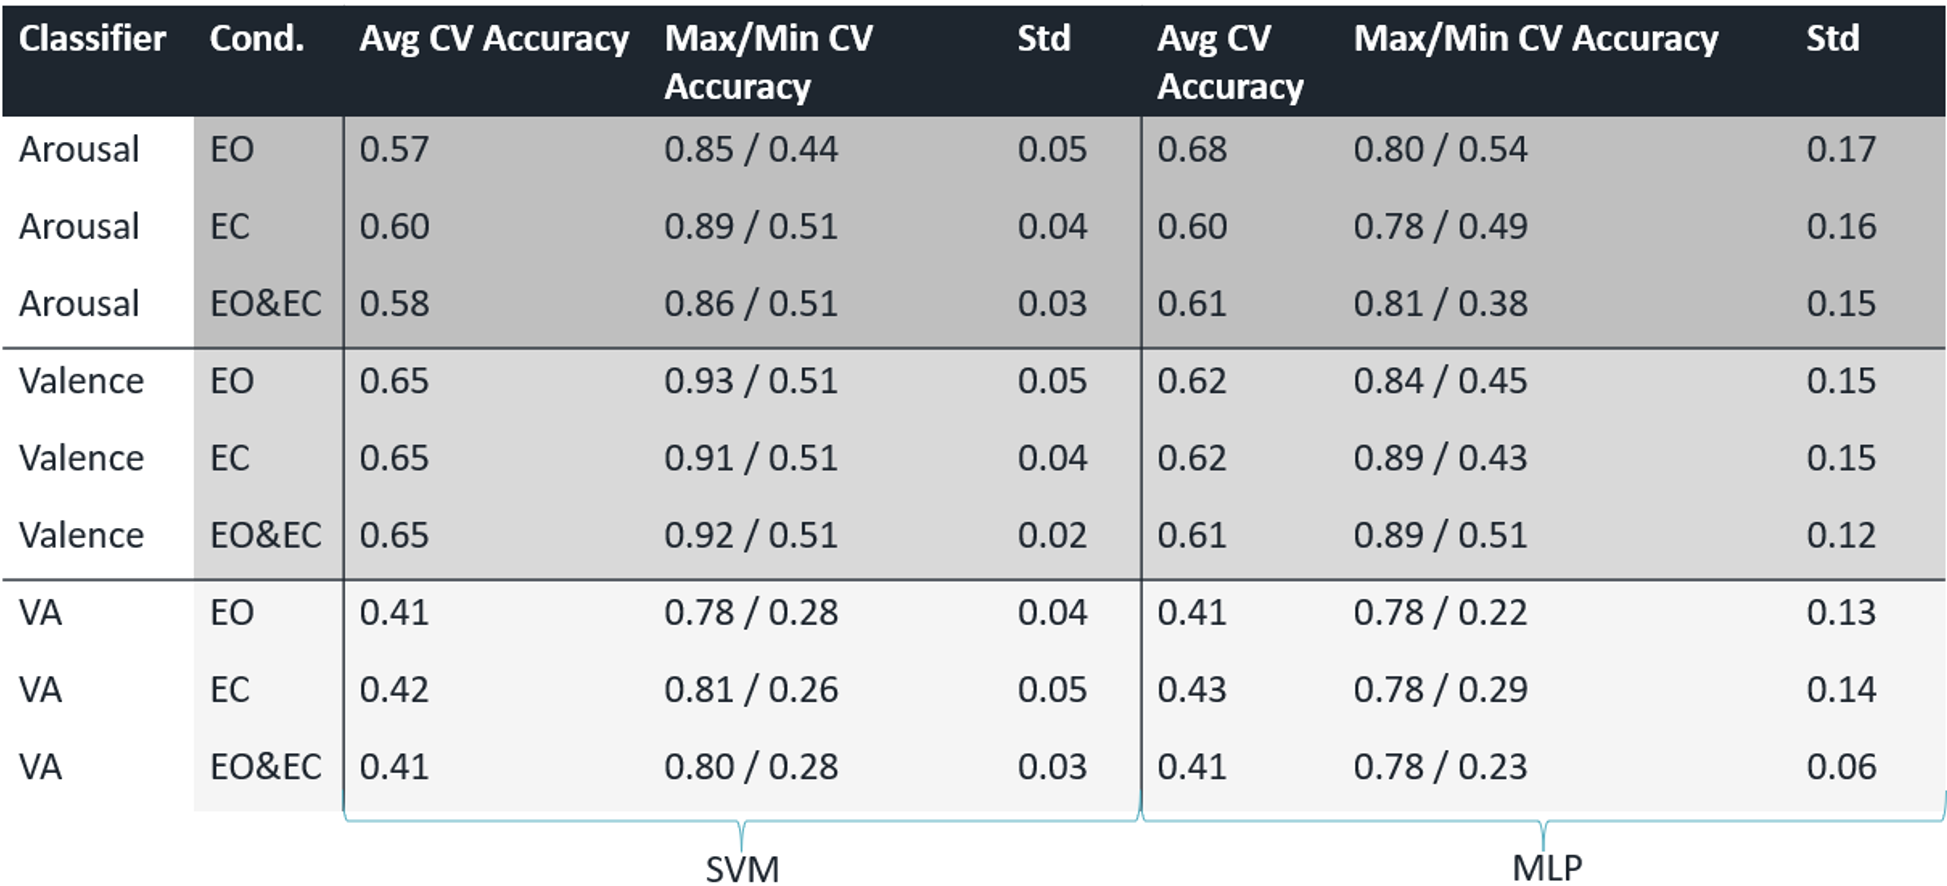
\includegraphics[width=\linewidth]{img/appendix/top5_cv_experiment.png}
\end{table}

\FloatBarrier
\subsection{Example of unbalanced dataset for arousal classification}
\label{sec:appendix_A3.3}
A more insightful study was conducted on participants with suspiciously high Test accuracy and low CV accuracy to identify the causes. Here is reported an example from a participant with unbalanced arousal labels. First, the labelling behaviour during experimental trials is reported in figure \ref{fig:arousal_unbalanced}, then the total distribution of \ac{VA} classes is reported in figure \ref{fig:arousal_unbalanced_distribution}.

\begin{figure}[!htb]
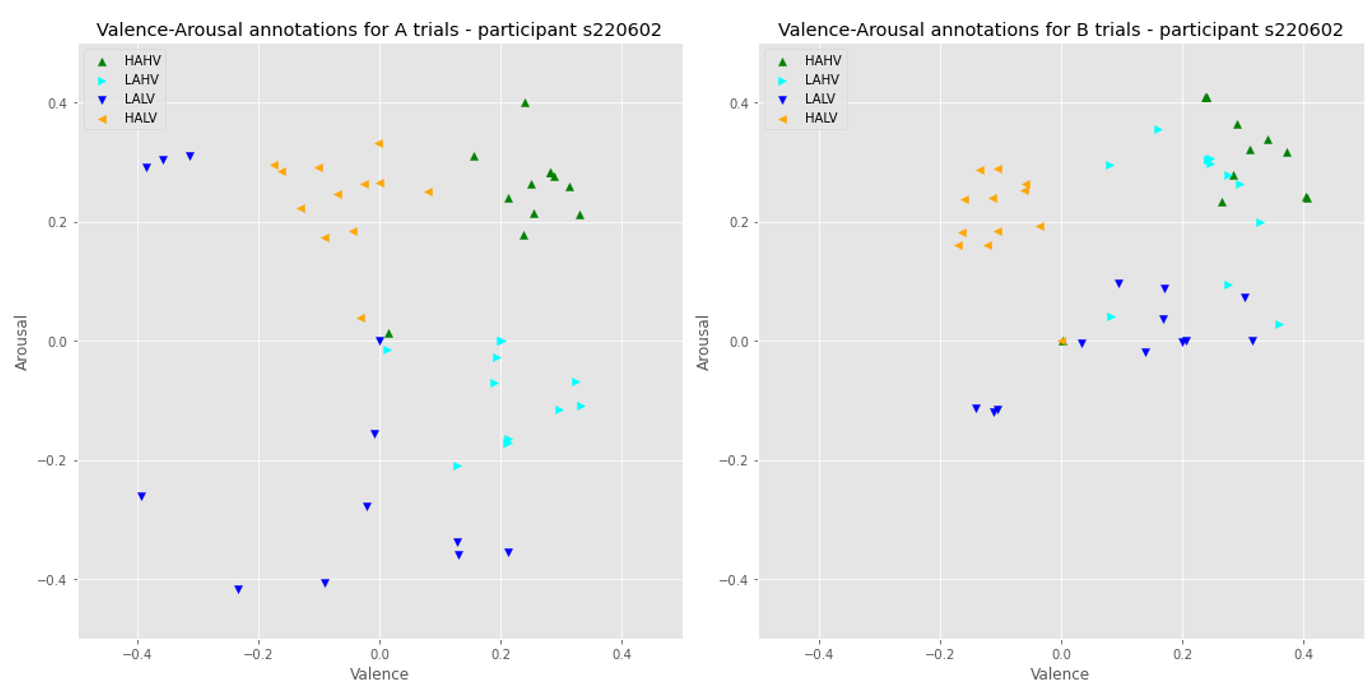
\includegraphics[width=16cm]{img/appendix/arousal_unbalanced.png}
\centering
\caption{Summary of annotation session for participant s220602. The labels are color coded according to the pre-labelled 
VA class of each song.}\label{fig:arousal_unbalanced}
\end{figure}

\begin{figure}[!htb]
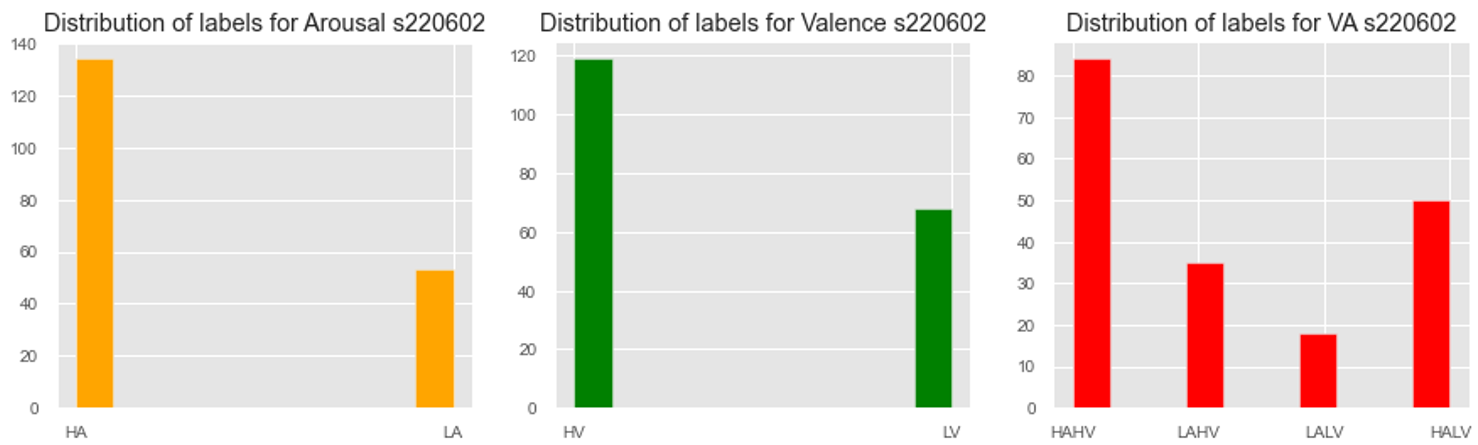
\includegraphics[width=16cm]{img/appendix/arousal_unbalanced_distribution.png}
\centering
\caption{Labels distribution of participant s220602. The LA* classes summed up are ~1/4 of the entire dataset.}\label{fig:arousal_unbalanced_distribution}
\end{figure}
\FloatBarrier
For both \ac{SVM} and \ac{MLP} classifiers cross-validated ROC curves were computed (see fig. \ref{fig:arousal_unbalanced_roc_svm} and fig. \ref{fig:arousal_unbalanced_roc_mlp}), showing the high variance between each split (in grey) against the mean accuracy (in blue), that is usually a symptom of overfitting.


\begin{figure}[!htb]
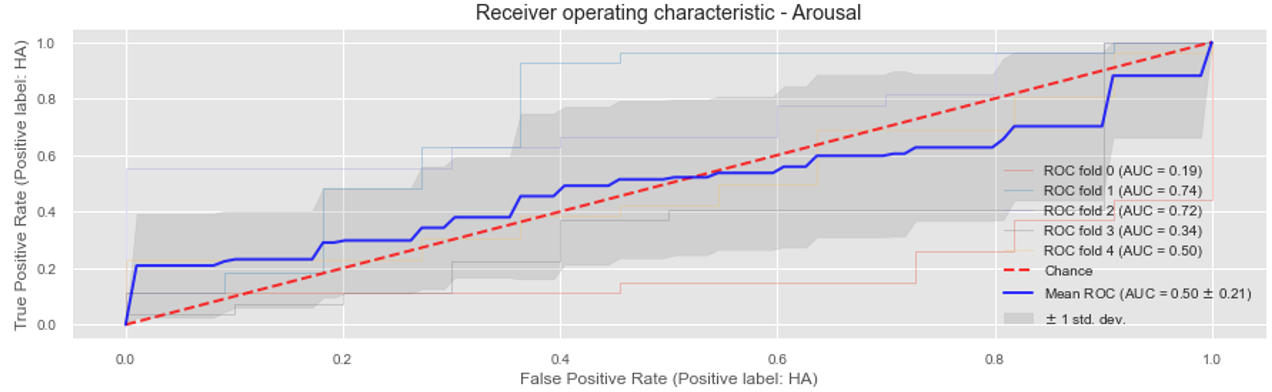
\includegraphics[width=16cm]{img/appendix/arousal_unbalanced_roc_svm.png}
\centering
\caption{Cross-validated ROC curve for participant s220602 for arousal classification using SVM.}\label{fig:arousal_unbalanced_roc_svm}
\end{figure}

\begin{figure}[!htb]
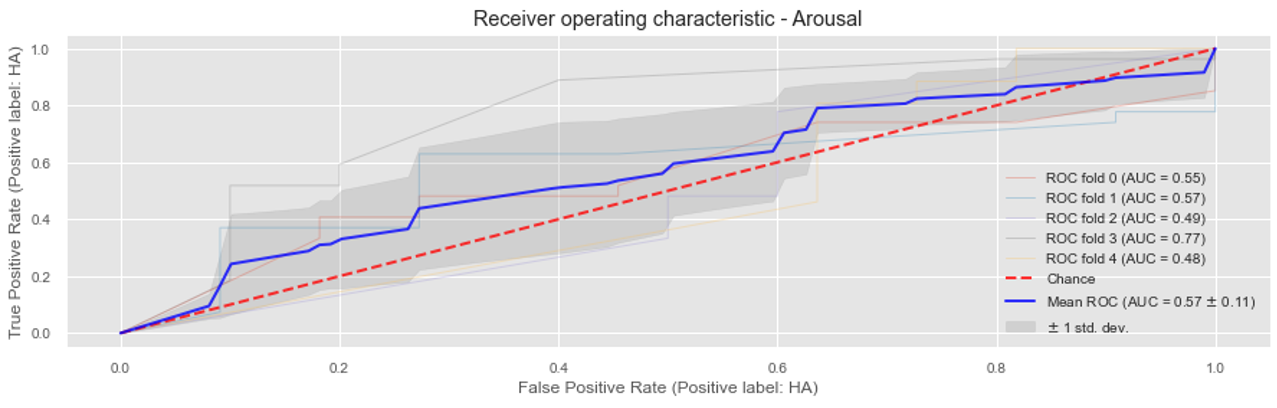
\includegraphics[width=16cm]{img/appendix/arousal_unbalanced_roc_mlp.png}
\centering
\caption{Cross-validated ROC curve for participant s220602 for arousal classification using MLP.}\label{fig:arousal_unbalanced_roc_mlp}
\end{figure}
\FloatBarrier
Finally, \ac{PCA} was computed to observe the distribution of labels across the first and the second principal components obtained by the features, and confusion matrices for both \ac{SVM} and \ac{MLP} revealed the difficulty in predicting the minority class due to the data not being linearly separable (see fig. \ref{fig:arousal_unbalanced_pca_confusion})

\begin{figure}[!htb]
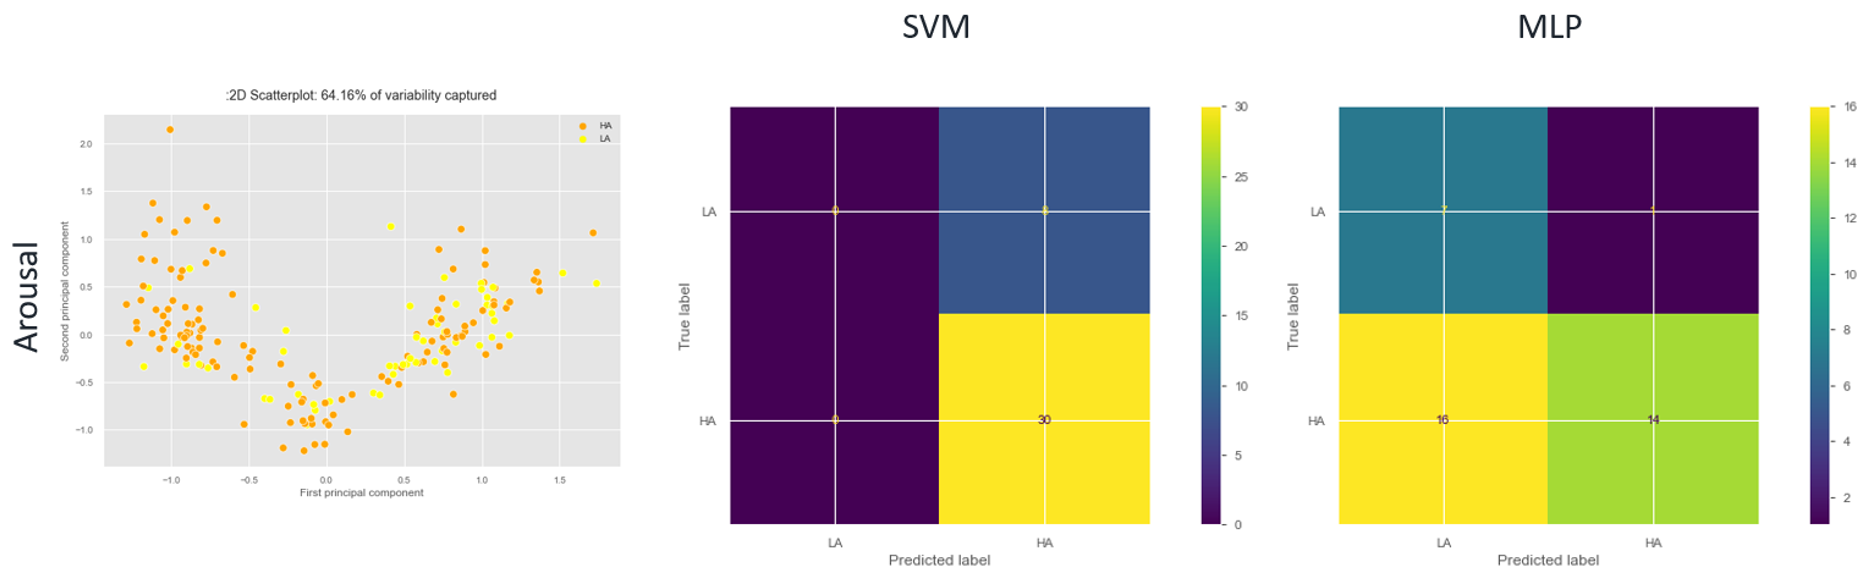
\includegraphics[width=16cm]{img/appendix/arousal_unbalanced_pca_confusion.png}
\centering
\caption{PCA (left) and confusion matrices (right) of s220602 participant with unbalanced labels for emotional arousal 
classification.}\label{fig:arousal_unbalanced_pca_confusion}
\end{figure}
\FloatBarrier
\subsection{Example of unbalanced dataset for valence classification}
\label{sec:appendix_A3.4}
A more insightful study was conducted on participants with suspiciously high Test accuracy and low CV accuracy to identify the causes. Here is reported an example from a participant with unbalanced valence labels. First, the labelling behaviour during experimental trials is reported in figure \ref{fig:valence_unbalanced}, then the total distribution of \ac{VA} classes is reported in figure \ref{fig:valence_unbalanced_distribution}.

\begin{figure}[!htb]
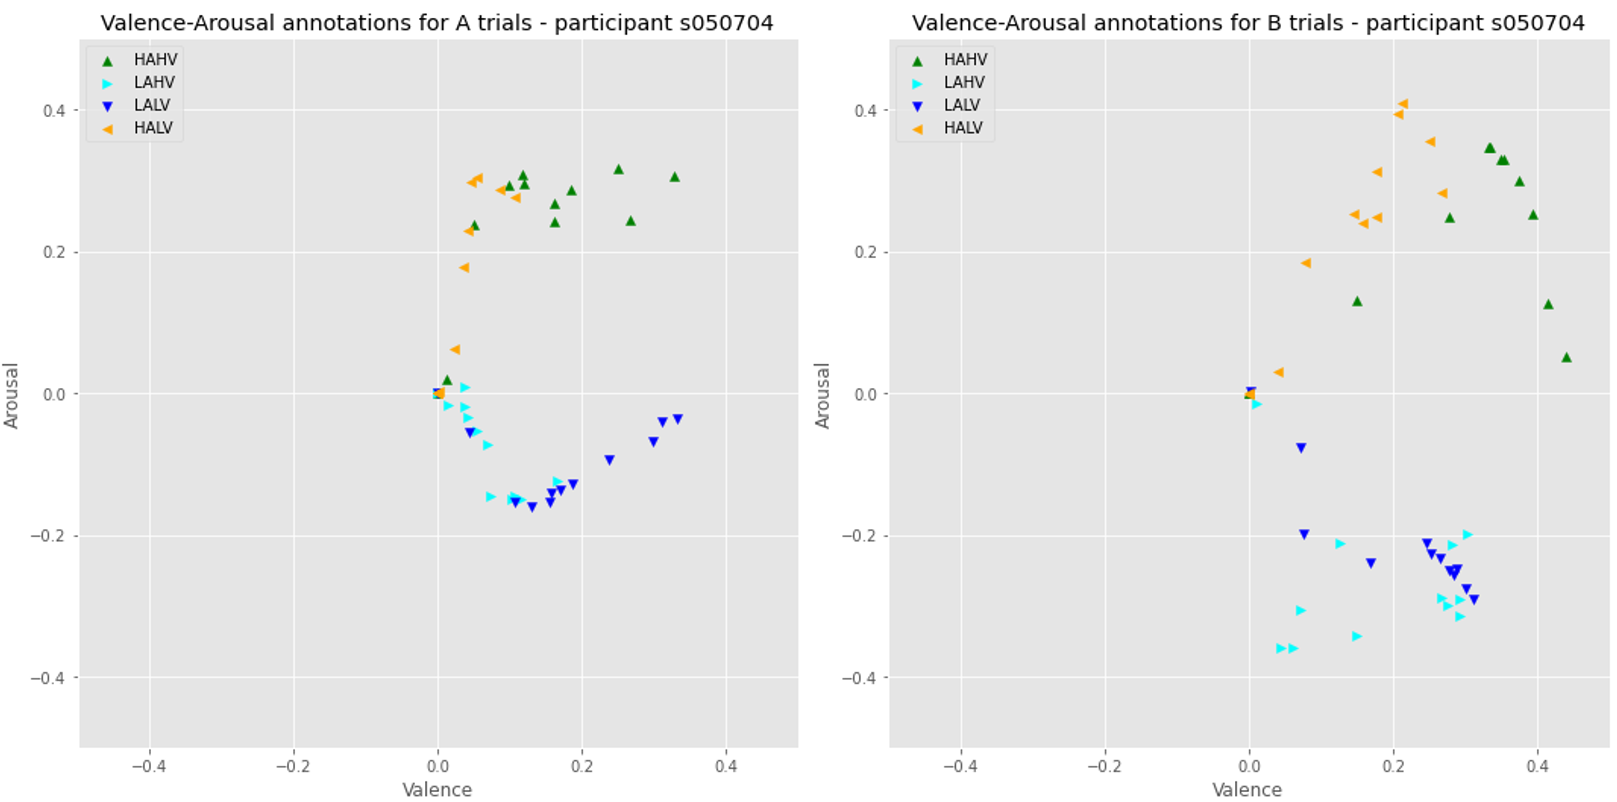
\includegraphics[width=16cm]{img/appendix/valence_unbalanced.png}
\centering
\caption{Summary of annotation session for participant s050704. The labels are color coded according to the pre-labelled 
VA class of each song.}\label{fig:valence_unbalanced}
\end{figure}

\begin{figure}[!htb]
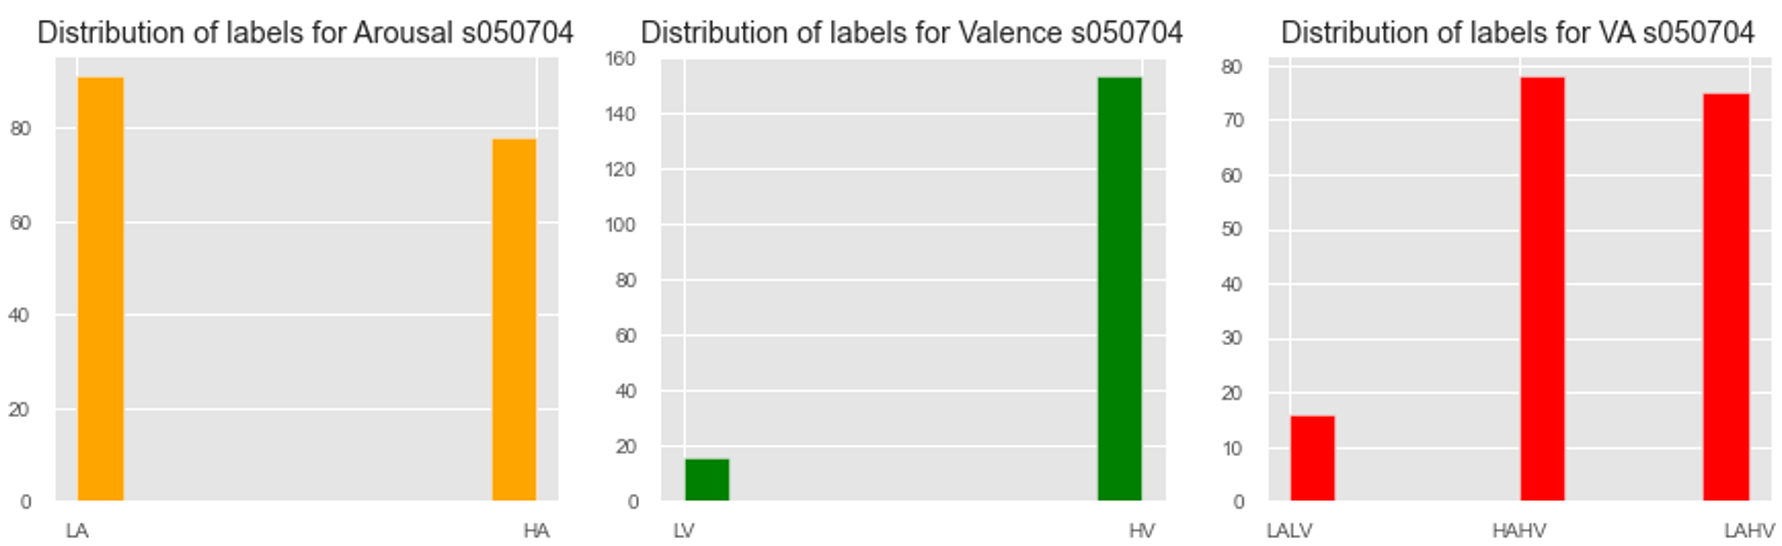
\includegraphics[width=16cm]{img/appendix/valence_unbalanced_distribution.png}
\centering
\caption{Labels distribution of participant s050704. The class HALV is completely missing.}\label{fig:valence_unbalanced_distribution}
\end{figure}
\FloatBarrier
For both \ac{SVM} and \ac{MLP} classifiers cross-validated ROC curves were computed (see fig. \ref{fig:valence_unbalanced_roc_svm} and fig. \ref{fig:valence_unbalanced_roc_mlp}), showing the high variance between each split (in grey) against the mean accuracy (in blue), that is usually a symptom of overfitting.


\begin{figure}[!htb]
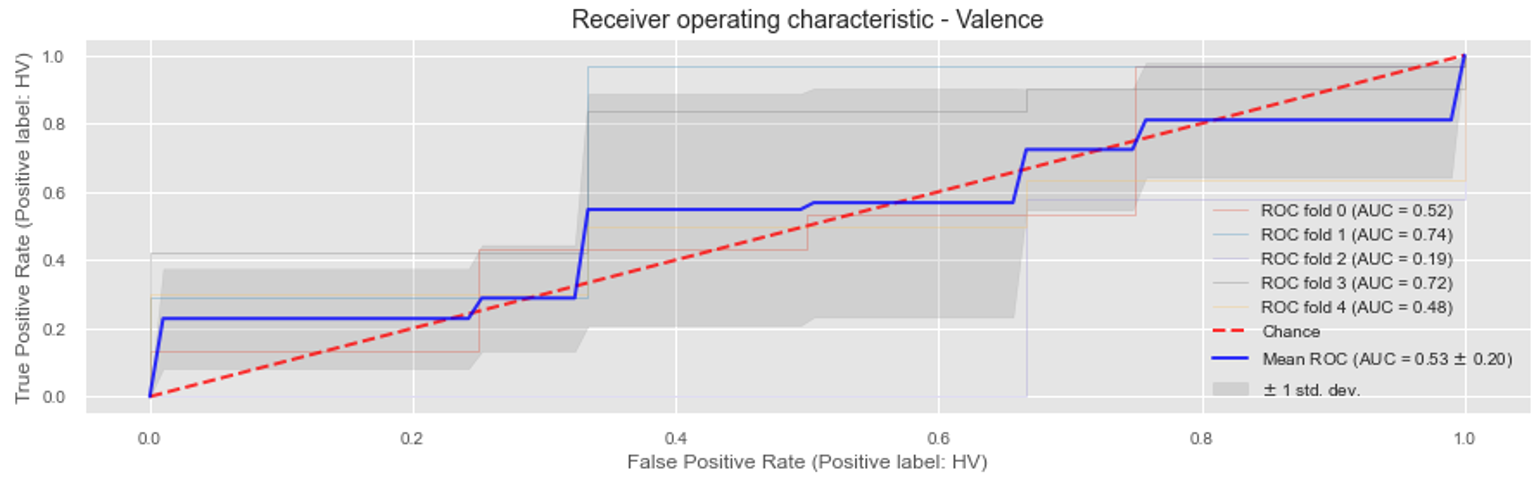
\includegraphics[width=16cm]{img/appendix/valence_unbalanced_roc_svm.png}
\centering
\caption{Cross-validated ROC curve for participant s050704 for valence classification using SVM.}\label{fig:valence_unbalanced_roc_svm}
\end{figure}

\begin{figure}[!htb]
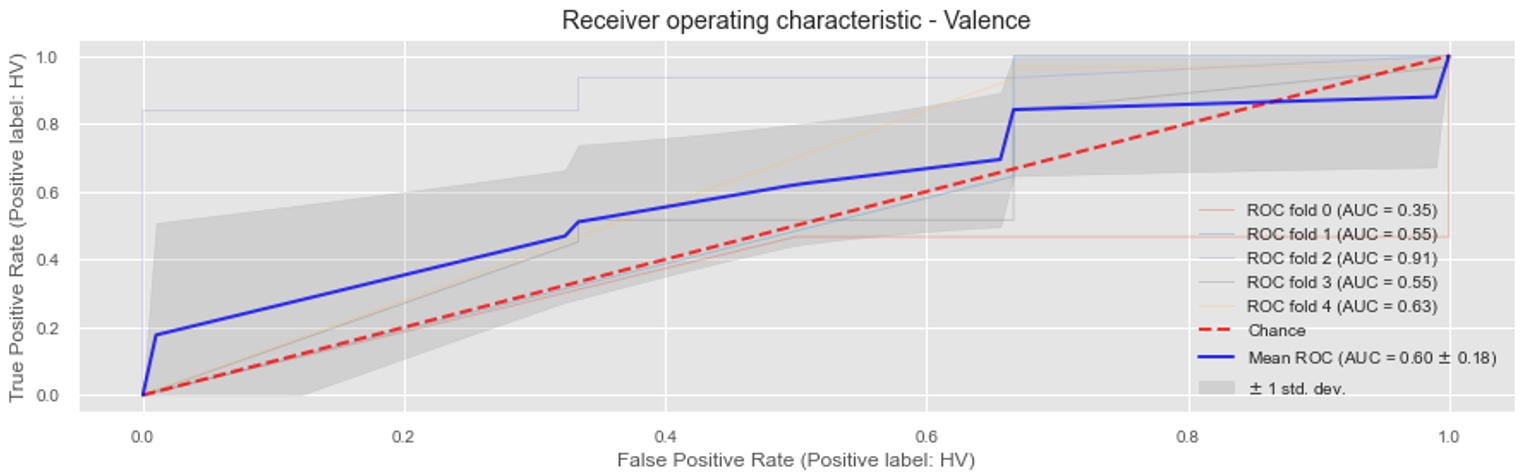
\includegraphics[width=16cm]{img/appendix/valence_unbalanced_roc_mlp.png}
\centering
\caption{Cross-validated ROC curve for participant s050704 for valence classification using MLP.}\label{fig:valence_unbalanced_roc_mlp}
\end{figure}
\FloatBarrier
Finally, \ac{PCA} was computed to observe the distribution of labels across the first and the second principal components obtained by the features, and confusion matrices for both \ac{SVM} and \ac{MLP} revealed the difficulty in predicting the minority class due to the data not being linearly separable (see fig. \ref{fig:valence_unbalanced_pca_confusion})

\begin{figure}[!htb]
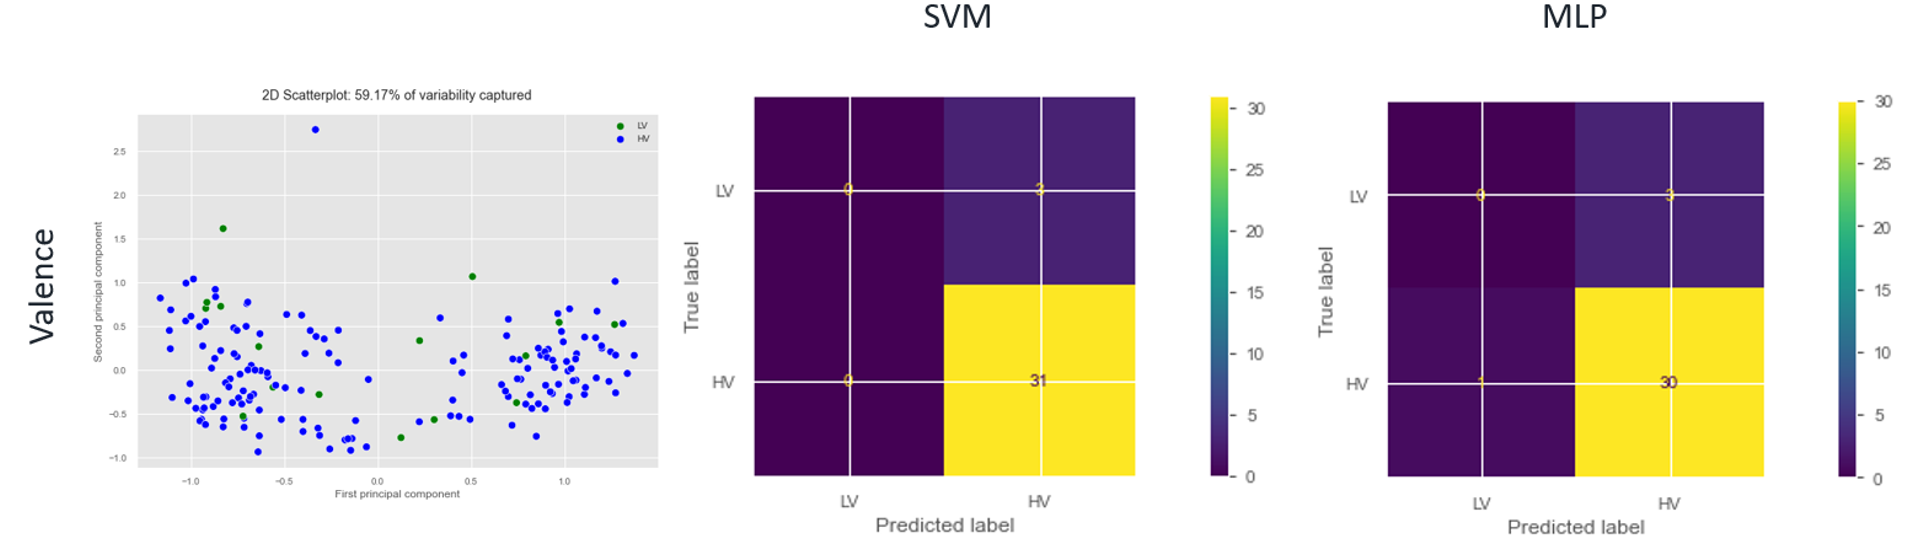
\includegraphics[width=16cm]{img/appendix/valence_unbalanced_pca_confusion.png}
\centering
\caption{PCA (left) and confusion matrices (right) of s050704 participant with unbalanced labels for emotional valence 
classification.}\label{fig:valence_unbalanced_pca_confusion}
\end{figure}
\FloatBarrier

\subsection{Subject-independent experiment with Top5 features}
\label{sec:appendix_A3.5}
Since it was impossible to apply \ac{SFS} to the entire dataset for subject-independent classification without days of computational time, for this experiment TOP5 features previously identified were used. The poor average results (see table \ref{tbl:top5_cv_si_experiment}) obtained pushed to focus this research on subject-dependent strategy. Another subject-independent experiment was conducted using \ac{PCA} on a sub-group of participants with balanced datasets, but the results were far below expectations and have not been saved for reporting.

\begin{table}[h!]
  \caption{ Average cross-validated accuracy for each classifier and listening condition using TOP5 features.}
  \label{tbl:top5_cv_si_experiment}
  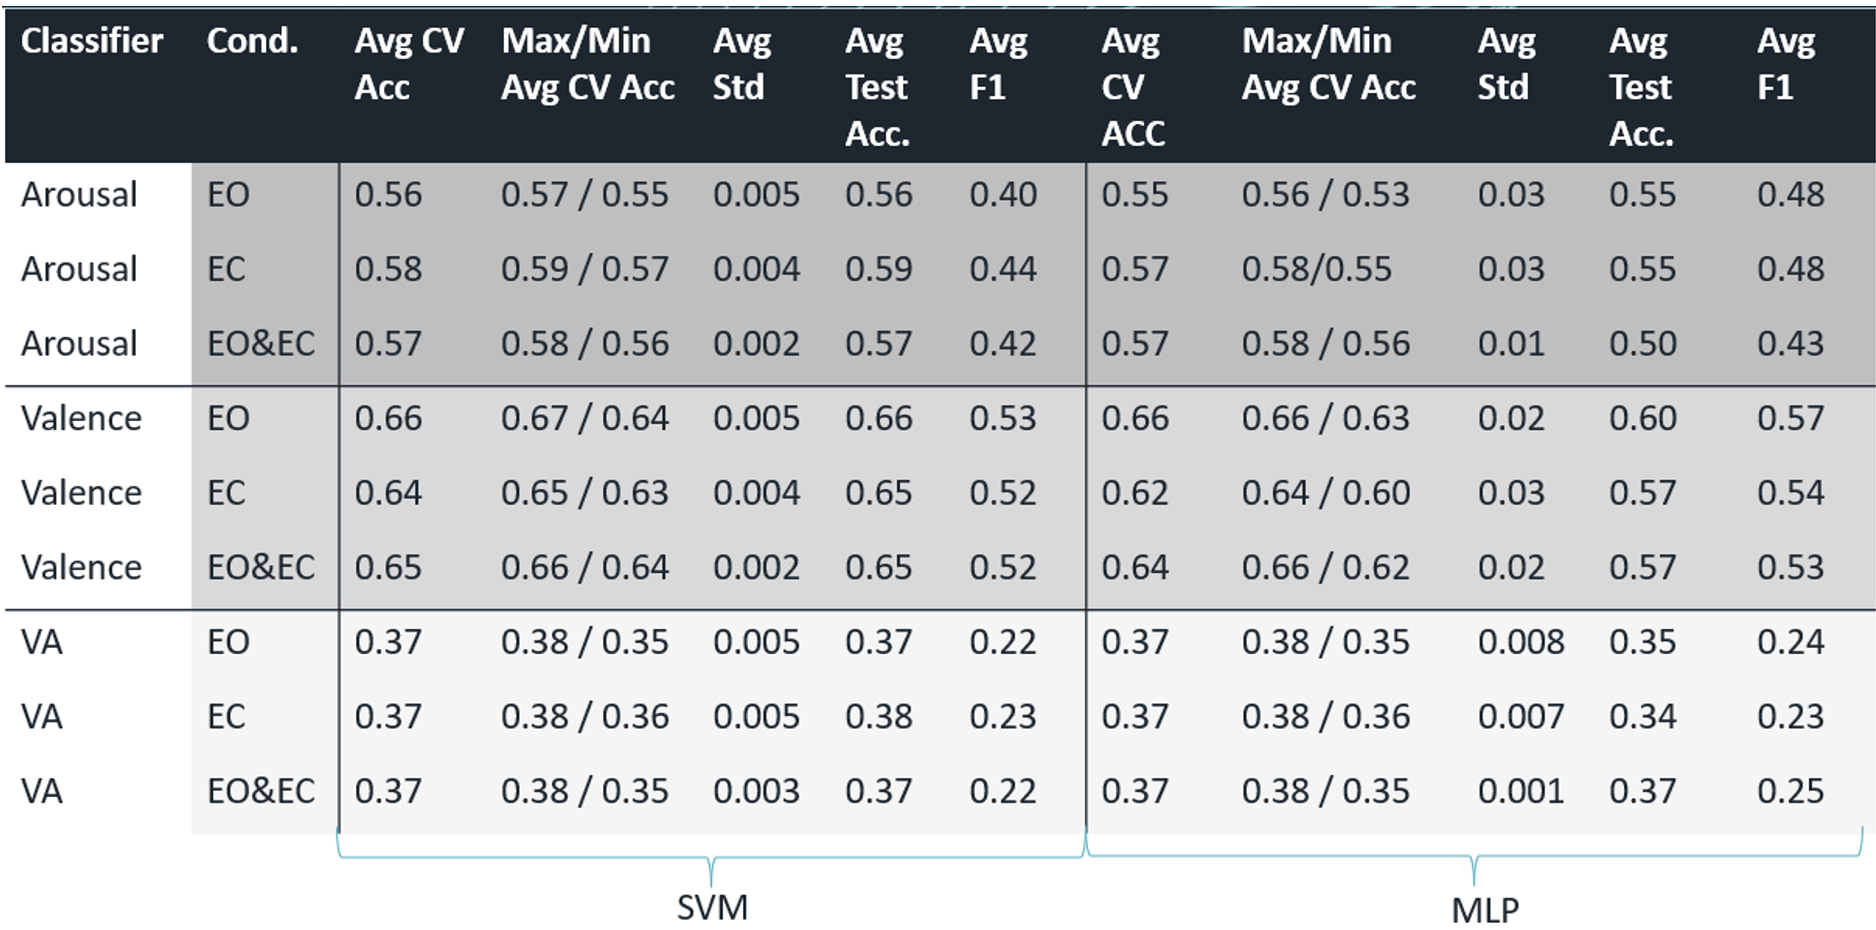
\includegraphics[width=\linewidth]{img/appendix/top5_cv_si_experiment.png}
\end{table}
\FloatBarrier

\subsection{Subject-dependent experiment with "Max Accuracy" scoring strategy}
\label{sec:appendix_A3.6}
Tables \ref{tbl:max_acc_arousal_results} and \ref{tbl:max_acc_valence_results} report the results for arousal and valence subject-dependent classification respectively with a scoring strategy that optimizes hyperparameters to maximize "accuracy" using GridSearch. While average accuracy and CV accuracy scores are higher, the number of overfitting and underfitting models that were generated, especially for \ac{SVM} classifier is also higher. This approach for GridSearch optimization was discarded in the final experiment in favor of maximising \ac{MCC} scores instead.
\begin{table}[h!]
  \caption{Arousal classification results using "accuracy" as scoring parameter for GridSearch. Learning models are highlighted in blue, over-fitted and under-fitted models are highlighted in yellow and orange, respectively.}
  \label{tbl:max_acc_arousal_results}
  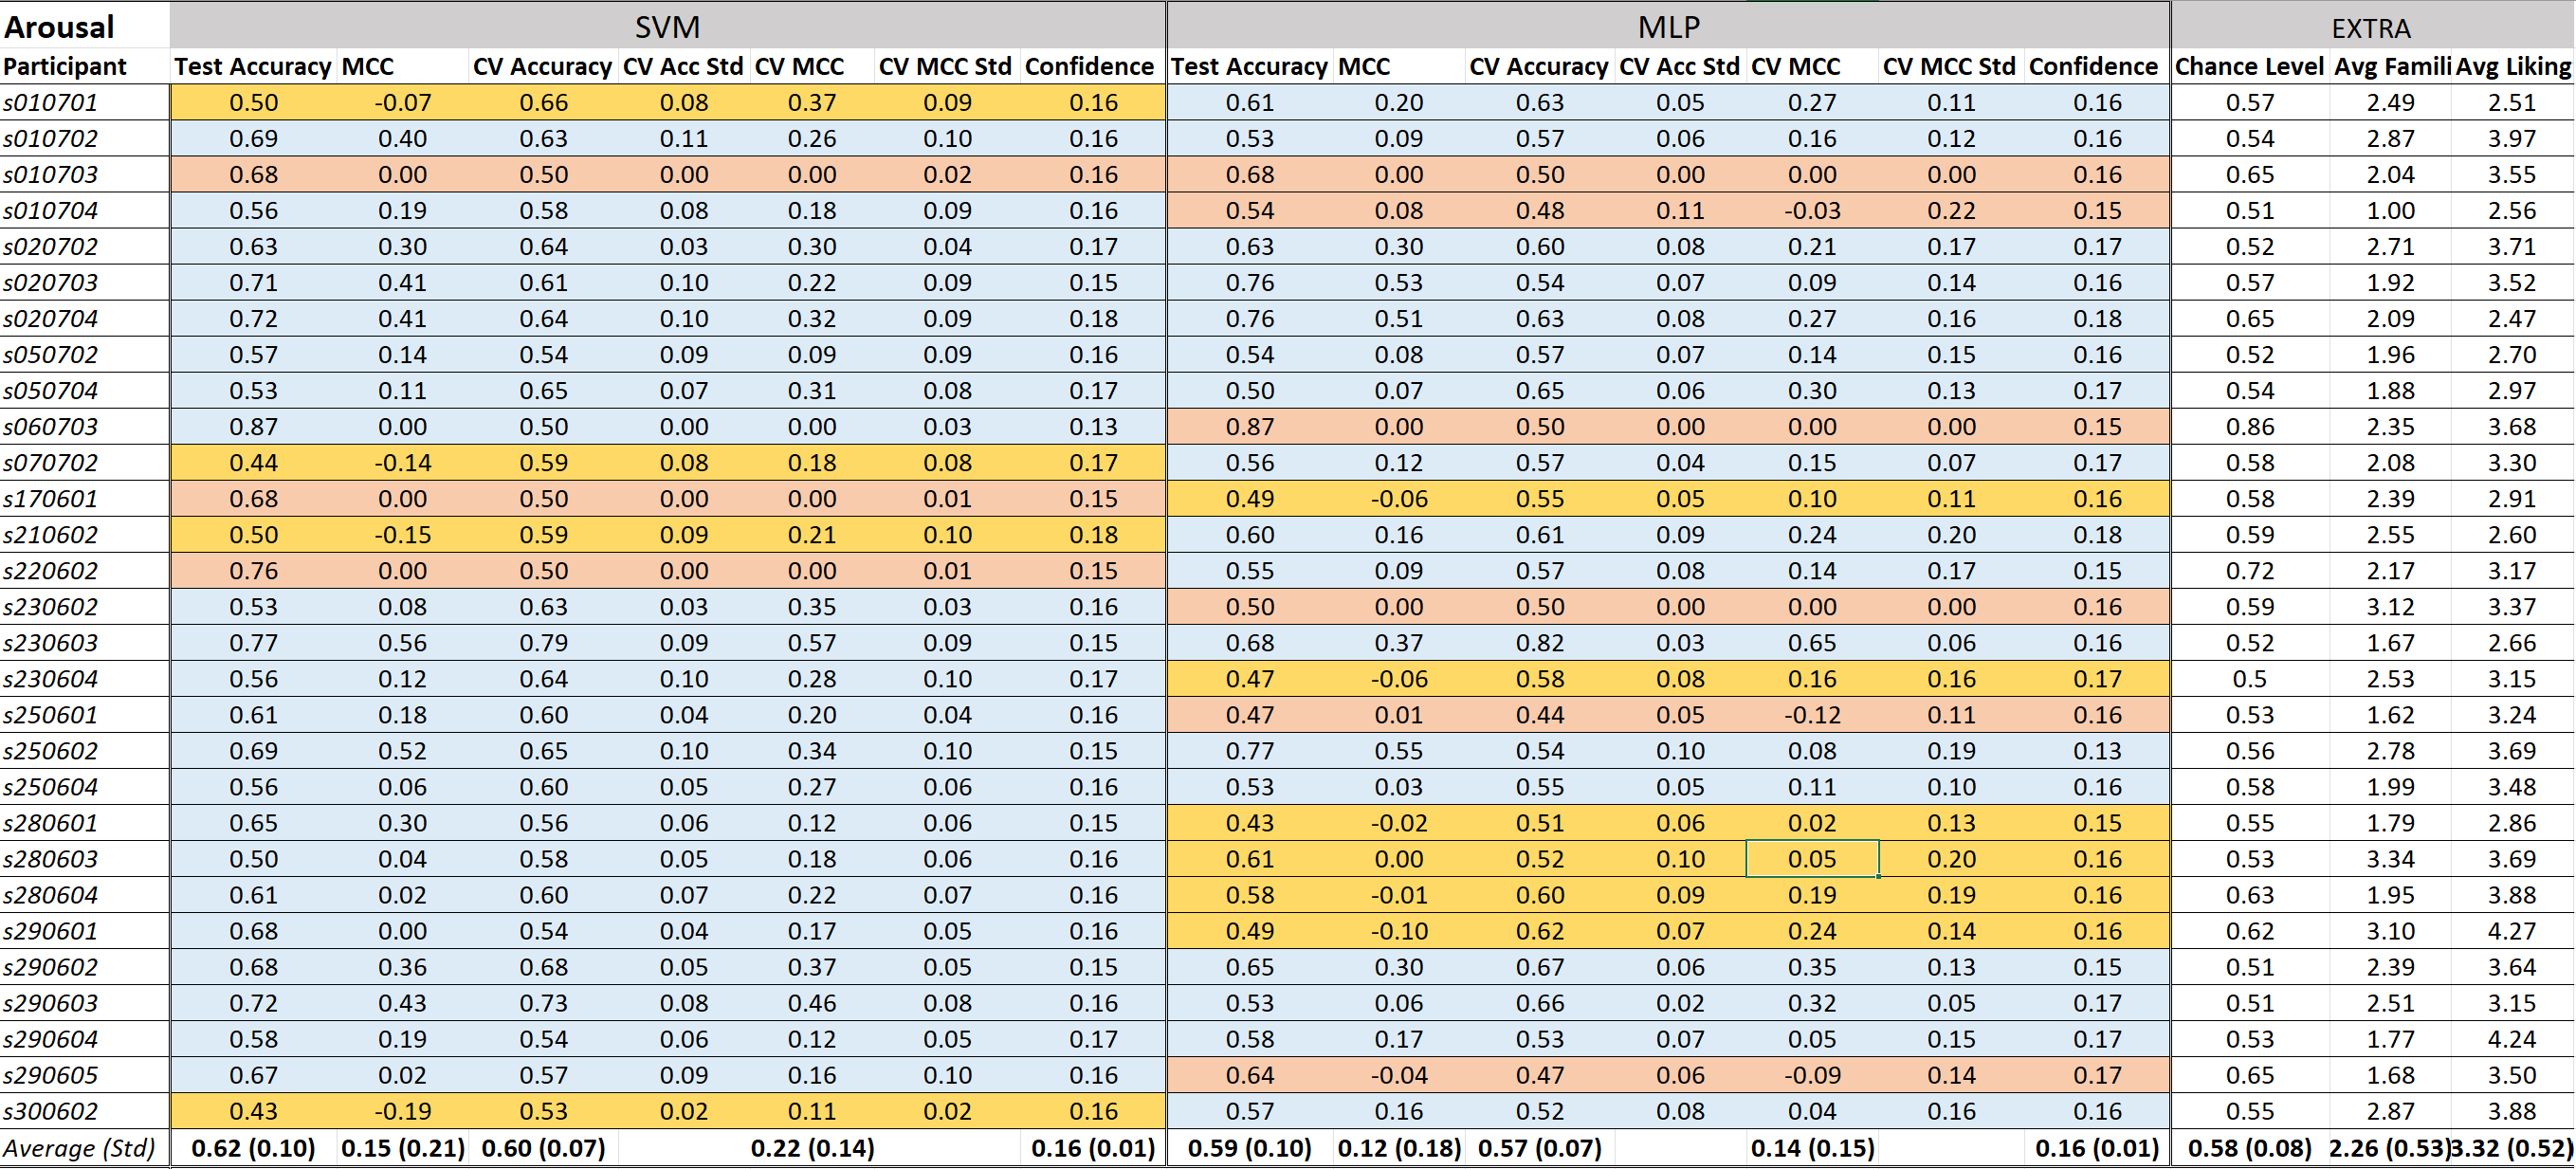
\includegraphics[width=\linewidth]{img/appendix/arousal_max_acc_results.png}
\end{table}

\begin{table}[h!]
  \caption{Valence classification results using "accuracy" as scoring parameter for GridSearch. Learning models are highlighted in blue, over-fitted and under-fitted models are highlighted in yellow and orange, respectively.}
  \label{tbl:max_acc_valence_results}
  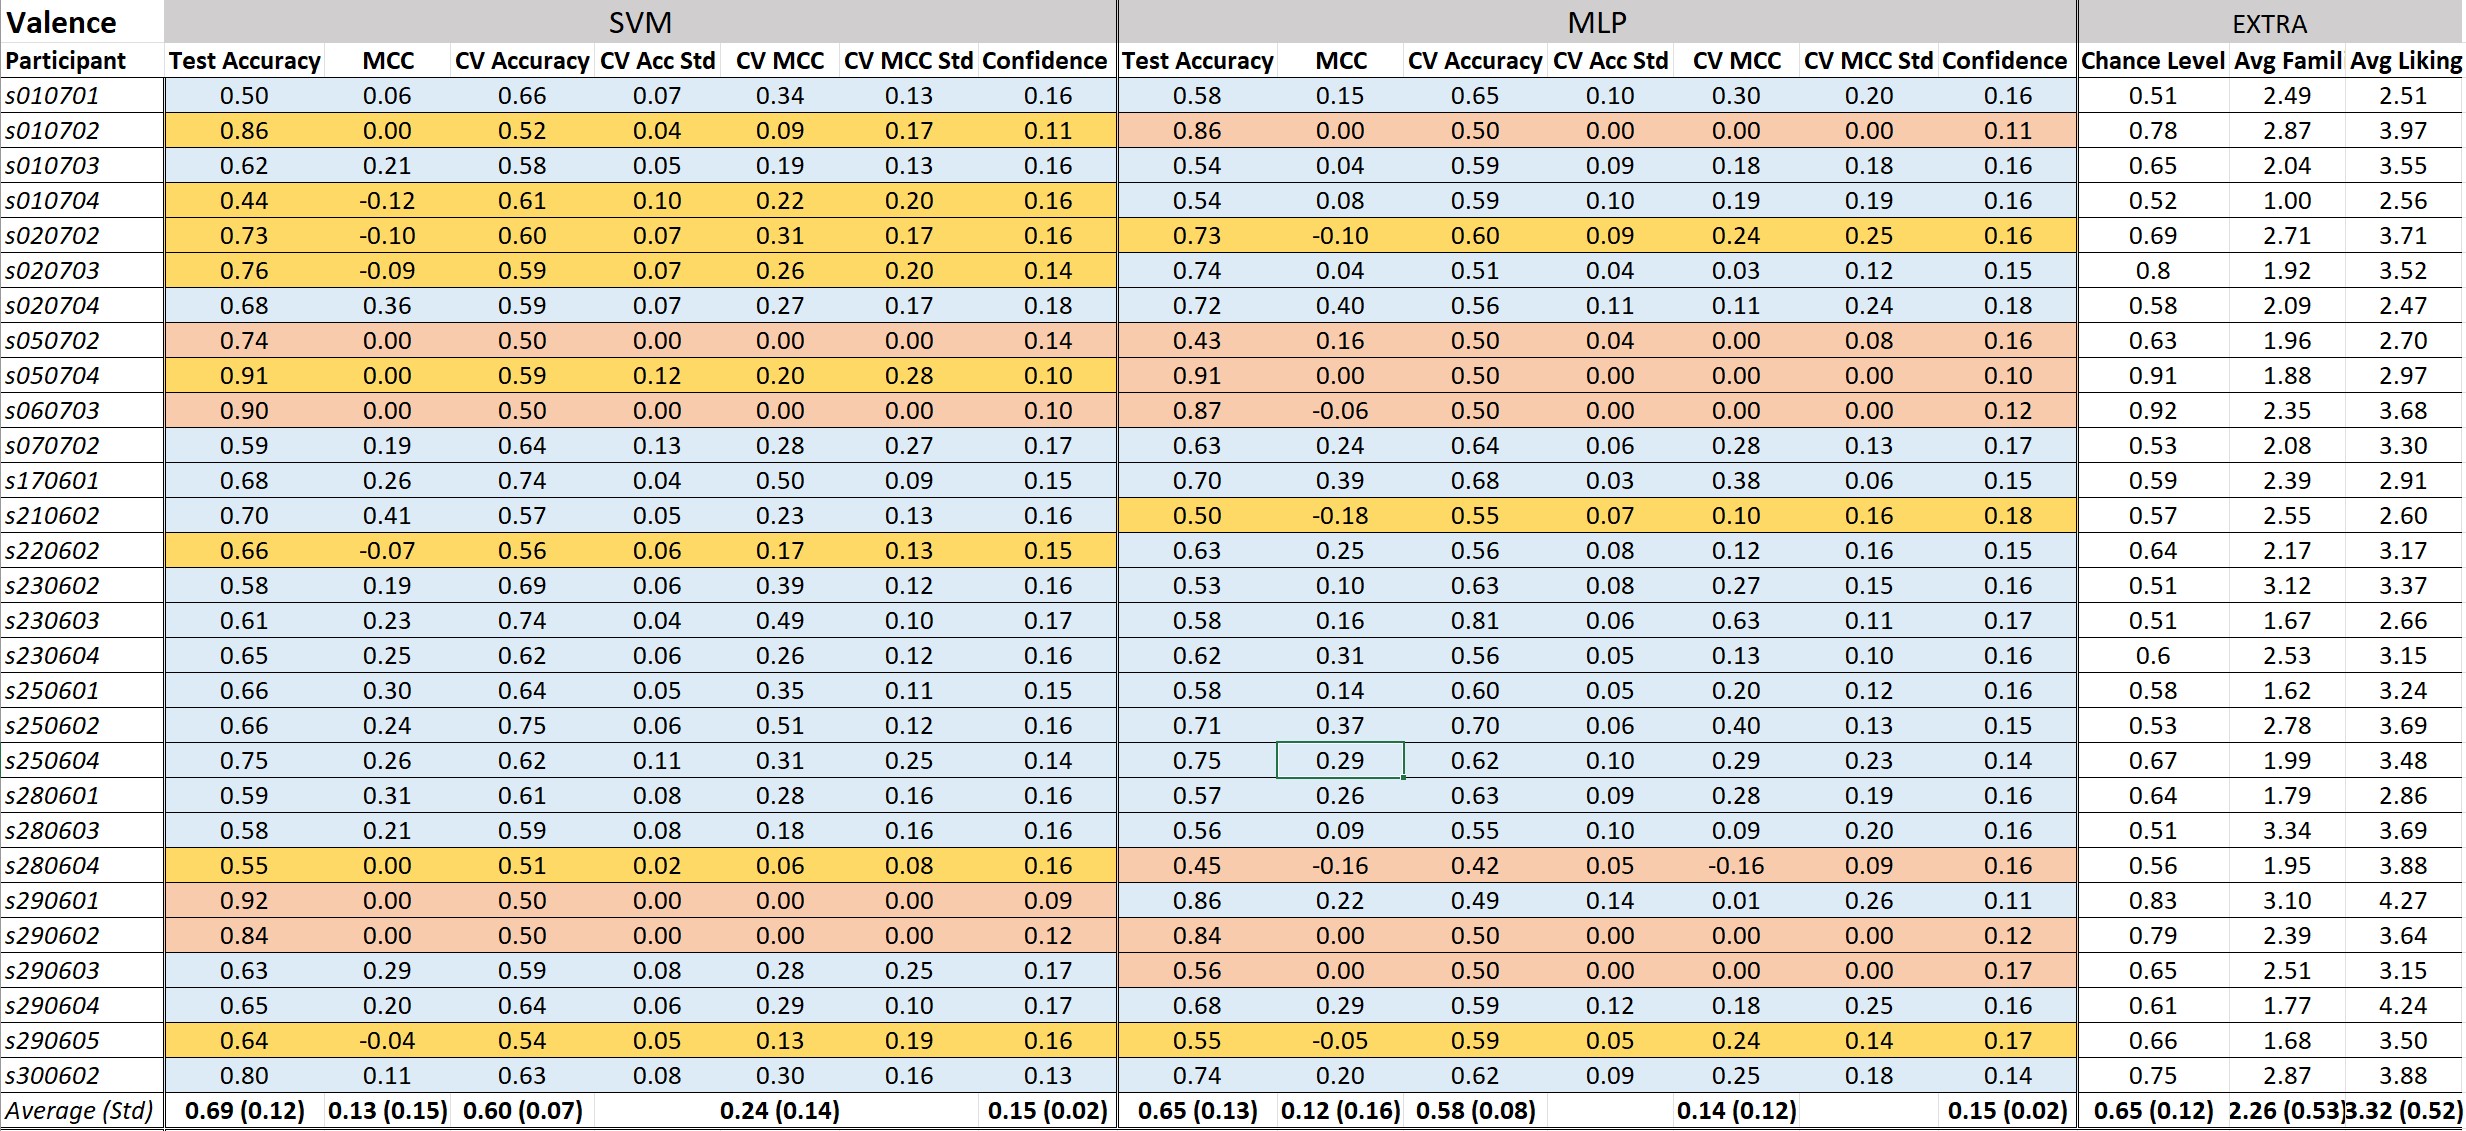
\includegraphics[width=\linewidth]{img/appendix/valence_max_acc_results.png}
\end{table}


\section{Final experiment}
\label{sec:appendix_A4}
The Test accuracy and \ac{MCC} scores of the final experiment with subject-dependent strategy have been averaged and compared with default guessing of the majority class in fig \ref{fig:experiment_test_recap}, while the cross-validated scores have been averaged and compared in fig. \ref{fig:experiment_cv_recap}. As it can be observed, the average accuracy scores are not significantly different than default guessing, but it should be considered that the maximization of \ac{MCC} scores often sacrifices accuracy when datasets have unbalanced labelling.


\begin{figure}[!htb]
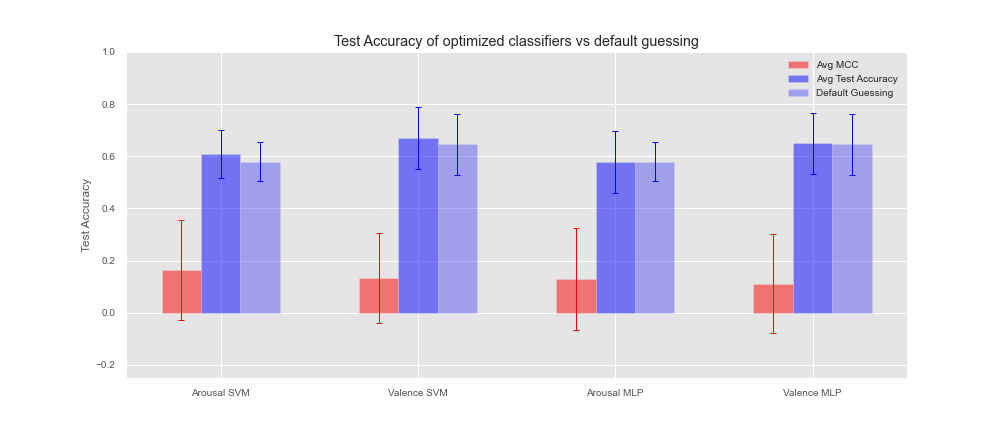
\includegraphics[width=16cm]{img/appendix/final_experiment/experiment_test_recap.png}
\centering
\caption{Average Test Accuracy and MCC compare against majority class guessing.}\label{fig:experiment_test_recap}
\end{figure}

\begin{figure}[!htb]
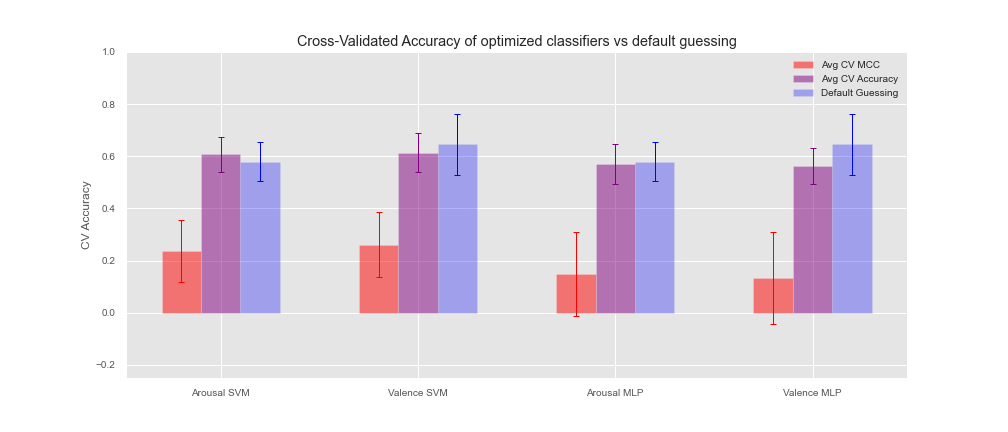
\includegraphics[width=16cm]{img/appendix/final_experiment/experiment_cv_recap.png}
\centering
\caption{Average CV Accuracy and CV MCC compare against majority class guessing.}\label{fig:experiment_cv_recap}
\end{figure}
\FloatBarrier

\subsection{Ranking of SVM classification performances for arousal classification}
\label{sec:appendix_A4.1}
Test accuracy and \ac{MCC} scores for arousal classification with \ac{SVM} have been ranked by descending \ac{MCC} (see fig. \ref{fig:test_acc_mcc_arousal_svm}), CV accuracy and \ac{CV MCC} have been ranked by descending \ac{CV MCC} (see fig. \ref{fig:test_cv_acc_mcc_arousal_svm}), and compared with default guessing for each participant. These ranking shows that the highest accuracy scores are often caused by unbalanced datasets. 


\begin{figure}[!htb]
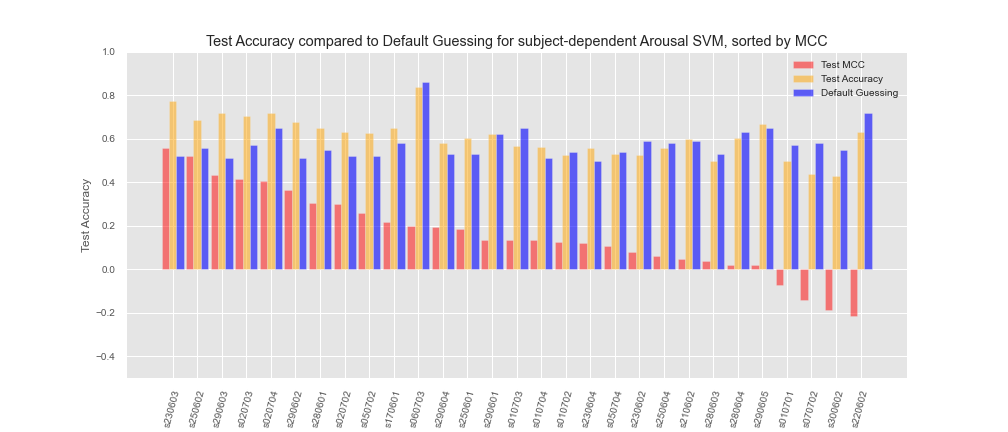
\includegraphics[width=16cm]{img/appendix/final_experiment/test_acc_mcc_arousal_svm.png}
\centering
\caption{Ranking of subject-dependent SVM models performances for arousal classification by Test MCC, descending.}\label{fig:test_acc_mcc_arousal_svm}
\end{figure}

\begin{figure}[!htb]
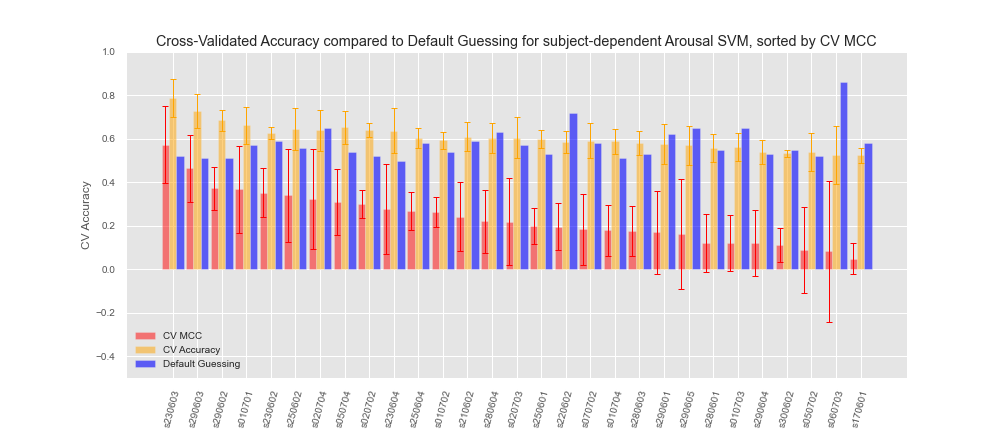
\includegraphics[width=16cm]{img/appendix/final_experiment/test_cv_acc_mcc_arousal_svm.png}
\centering
\caption{Ranking of subject-dependent SVM models performances for arousal classification by CV MCC, descending.}\label{fig:test_cv_acc_mcc_arousal_svm}
\end{figure}
\FloatBarrier

\subsection{Ranking of MLP classification performances for arousal classification}
\label{sec:appendix_A4.2}
Test accuracy and \ac{MCC} scores for arousal classification with \ac{MLP} have been ranked by descending \ac{MCC} (see fig. \ref{fig:test_acc_mcc_arousal_mlp}), CV accuracy and \ac{CV MCC} have been ranked by descending \ac{CV MCC}, and compared with default guessing for each participant (see fig. \ref{fig:test_cv_acc_mcc_arousal_mlp}). These ranking shows that the highest accuracy scores are often caused by unbalanced datasets. 

\begin{figure}[!htb]
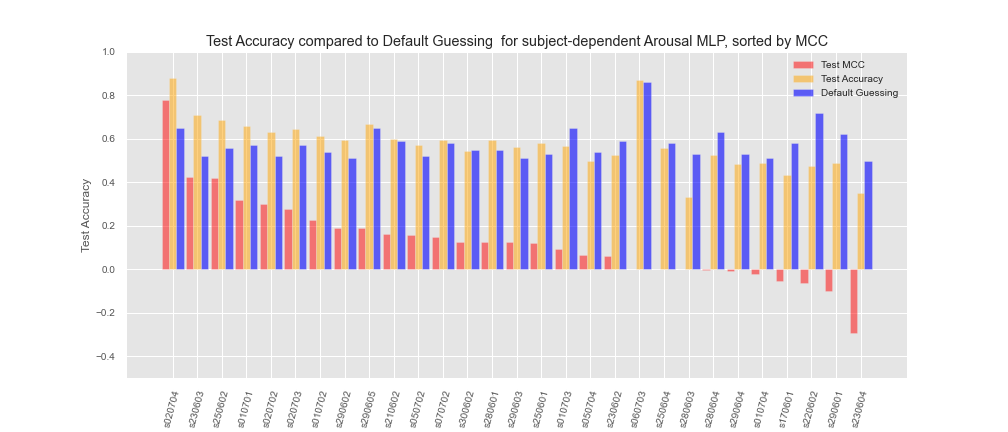
\includegraphics[width=16cm]{img/appendix/final_experiment/test_acc_mcc_arousal_mlp.png}
\centering
\caption{Ranking of subject-dependent MLP models performances for arousal classification by Test MCC, descending.}\label{fig:test_acc_mcc_arousal_mlp}
\end{figure}

\begin{figure}[!htb]
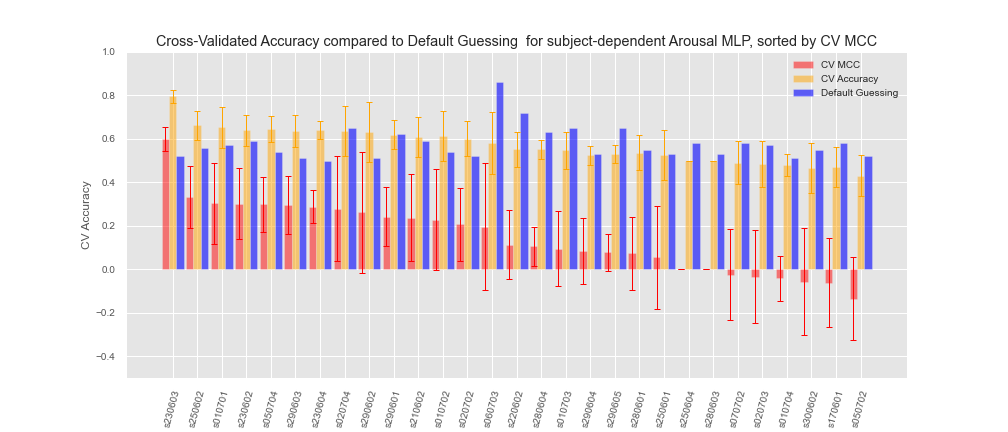
\includegraphics[width=16cm]{img/appendix/final_experiment/test_cv_acc_mcc_arousal_mlp.png}
\centering
\caption{Ranking of subject-dependent MLP models performances for arousal classification by CV MCC, descending.}\label{fig:test_cv_acc_mcc_arousal_mlp}
\end{figure}
\FloatBarrier

\subsection{Ranking of SVM classification performances for valence classification}
\label{sec:appendix_A4.3}
Test accuracy and \ac{MCC} scores for valence classification with \ac{SVM} have been ranked by descending \ac{MCC} (see fig. \ref{fig:test_acc_mcc_valence_svm}), CV accuracy and \ac{CV MCC} have been ranked by descending \ac{CV MCC} (see fig. \ref{fig:test_cv_acc_mcc_valence_svm}), and compared with default guessing for each participant. These ranking shows that the highest accuracy scores are often caused by unbalanced datasets. 

\begin{figure}[!htb]
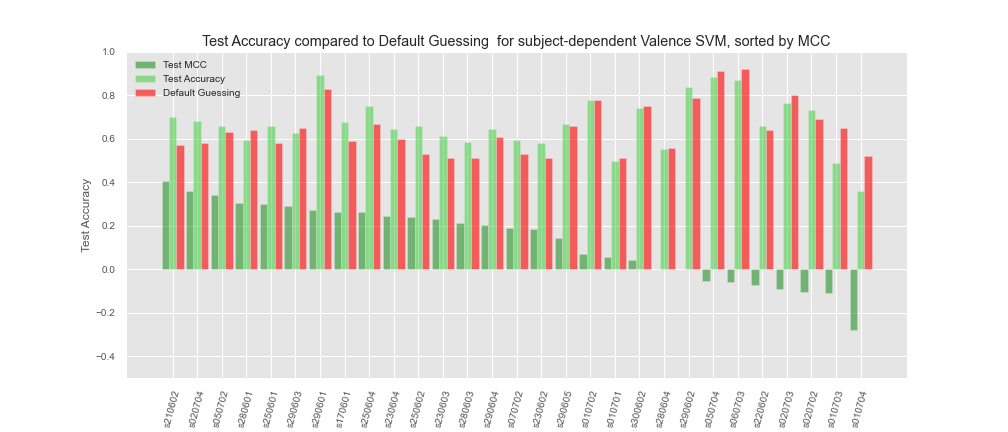
\includegraphics[width=16cm]{img/appendix/final_experiment/test_acc_mcc_valence_svm.png}
\centering
\caption{Ranking of subject-dependent SVM models performances for valence classification by Test MCC, descending.}\label{fig:test_acc_mcc_valence_svm}
\end{figure}

\begin{figure}[!htb]
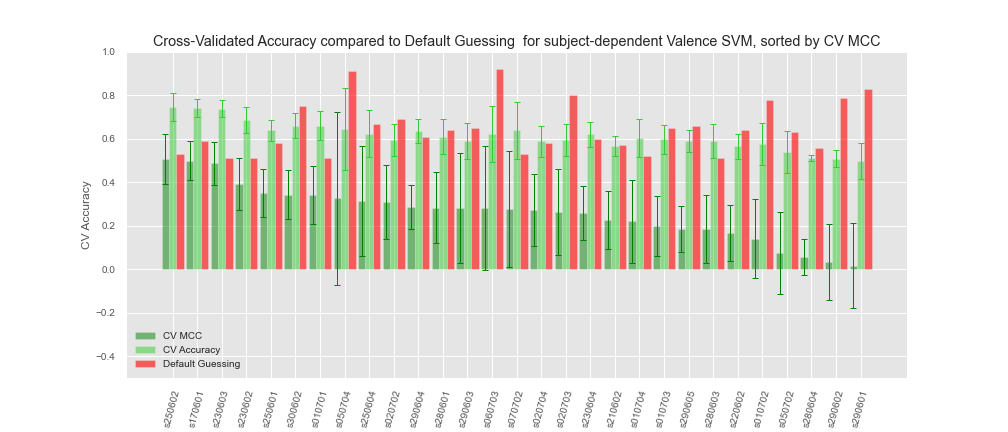
\includegraphics[width=16cm]{img/appendix/final_experiment/test_cv_acc_mcc_valence_svm.png}
\centering
\caption{Ranking of subject-dependent SVM models performances for valence classification by CV MCC, descending.}\label{fig:test_cv_acc_mcc_valence_svm}
\end{figure}
\FloatBarrier

\subsection{Ranking of MLP classification performances for valence classification}
\label{sec:appendix_A4.4}
Test accuracy and \ac{MCC} scores for valence classification with \ac{SVM} have been ranked by descending \ac{MCC} (see fig. \ref{fig:test_acc_mcc_valence_mlp}), CV accuracy and \ac{CV MCC} have been ranked by descending \ac{CV MCC} (see fig. \ref{fig:test_cv_acc_mcc_valence_mlp}), and compared with default guessing for each participant. These ranking shows that the highest accuracy scores are often caused by unbalanced datasets. 

\begin{figure}[!htb]
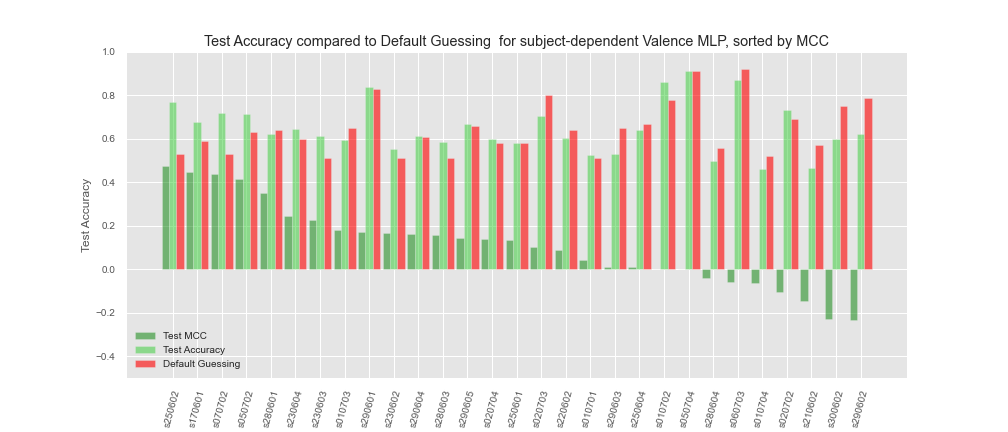
\includegraphics[width=16cm]{img/appendix/final_experiment/test_acc_mcc_valence_mlp.png}
\centering
\caption{Ranking of subject-dependent MLP models performances for valence classification by Test MCC, descending.}\label{fig:test_acc_mcc_valence_mlp}
\end{figure}

\begin{figure}[!htb]
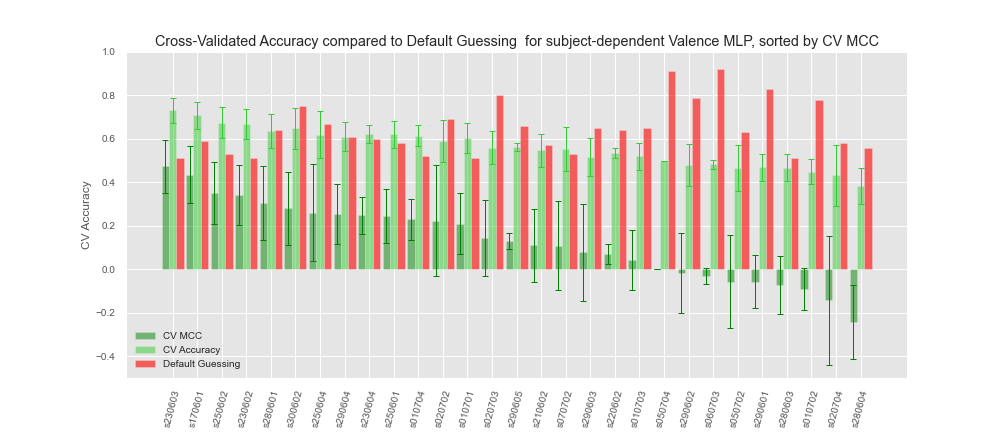
\includegraphics[width=16cm]{img/appendix/final_experiment/test_cv_acc_mcc_valence_mlp.png}
\centering
\caption{Ranking of subject-dependent MLP models performances for valence classification by CV MCC, descending.}\label{fig:test_cv_acc_mcc_valence_mlp}
\end{figure}
